\documentclass[12pt,oneside,a4paper]{bookAnh1}
\usepackage[utf8]{vietnam}
\usepackage{amsmath}
\usepackage[colorlinks=true]{hyperref}
\hypersetup{urlcolor=red, citecolor=blue,linkcolor=blue} %Itemize
%\usepackage{subfig}
\usepackage{longtable,mathrsfs,cite}
\usepackage{makecell}
\usepackage{graphicx}
\usepackage{fancybox}
\usepackage{subfigure}
\usepackage{inputenc}
\usepackage{hyperref}
\usepackage{algorithm}
\usepackage{algorithmicx}
\usepackage{algpseudocode}
\usepackage{amsfonts}
\usepackage{amssymb}
\usepackage{titlesec}
\usepackage{graphicx,xcolor}
\usepackage{tikz}
\usetikzlibrary{shapes.geometric,arrows,calc,intersections,angles,patterns,snakes,positioning}
\usepackage{titlesec}
\usepackage{mdframed}
\usepackage[top=2cm, bottom=2cm, left=3cm, right=2cm] {geometry}
\def \baselinestretch{1.5}
\usepackage{enumerate} %Enumerate
\usepackage[shortlabels]{enumitem}

% %%%%%%%%%%%%ĐỊNH LÝ %%%%%%%%%%%%%%%%%%
%Theorem
%%%%%%%%%%%%%%%%%%%%%%%%

%%%%%%%%%%%%%%%%%%%%%%%%%%%%
\usepackage{multicol}
%%\usepackage{mathptmx}
%%\usepackage[left=2.5cm,right=2.5cm,top=2.5cm,bottom=2.5cm]{geometry}
%
%%\usepackage{titlesec}
%%\usepackage{mdframed}

\usepackage{titletoc} % Gói lệnh tùy chỉnh thêm chữ "Chương" ở mục lục
\titlecontents{chapter}% <section-type>
[0pt]% <left>
{\addvspace{1em}}% <above-code>
{\bfseries\chaptername\ \thecontentslabel.\ }% <numbered-entry-format>
{}% <numberless-entry-format>
{\bfseries\hfill\contentspage}% <filler-page-format>

%=========================================================
%Item
\usepackage{enumerate} %Enumerate
\usepackage[shortlabels]{enumitem} %Itemize
\usepackage{pgf,tikz}
\DeclareMathOperator{\gr}{gph}%
\DeclareMathOperator{\dom}{dom}
\DeclareMathOperator{\cl}{cl}
\DeclareMathOperator{\ptrog}{int}
\DeclareMathOperator{\dk}{diam}
\DeclareMathOperator{\lev}{lev}
\DeclareMathOperator{\wmin}{WMin}
\DeclareMathOperator{\weff}{WEff}
\DeclareMathOperator{\argmin}{argmin}
%\numberwithin{equation}{section}

\newenvironment{Oboxedminipage} {\begin{Sbox}\begin{minipage}} {\end{minipage}\end{Sbox} \Ovalbox{\TheSbox}}
%Space
\renewcommand{\baselinestretch}{1.5}
\setlength{\parindent}{0.5cm}
%\setlength\parskip{10pt}
\def\arraystretch{1.25}	%Adjusting space between array rows

%=========================================================
%Chapter, section, subsection,...
\usepackage[thref,thmmarks,standard,amsmath,hyperref]{ntheorem}
\theoremheaderfont{\normalfont\bfseries}
\theorembodyfont{\normalfont}
\theoremseparator{}

%Theorem
\theorembodyfont{\itshape}
\renewtheorem{theorem}{Định lý}[chapter]
\renewtheorem{proposition}{Mệnh đề}[chapter]
\renewtheorem{lemma}{Bổ đề}[chapter]
\renewtheorem{corollary}{Hệ quả}[chapter]
\newtheorem{assumption}{Giả thiết}
\theorembodyfont{\normalfont}
\renewtheorem{definition}{Định nghĩa}[chapter]
\renewtheorem{remark}{Nhận xét}[chapter]
\renewtheorem{example}{Ví dụ}[chapter]

%Proof
\theoremstyle{plain}
\theoremstyle{nonumberplain}
\theoremsymbol{\ensuremath{\square}}
\renewtheorem{proof}{Chứng minh.}

\usepackage{fancyhdr} % Gói lệnh tùy chỉnh Header & Footer
% IN 1 MẶT
\thispagestyle{plain}
\pagestyle{fancy}
\lhead{}
\chead{}
\rhead{}
%\rhead{\fontsize{10pt}{10pt}\selectfont\nouppercase{\leftmark}}
%\lfoot{\fontsize{10pt}{10pt}\selectfont\nouppercase{\rightmark}}
\cfoot{\thepage} % Chèn số trang
\rfoot{}
\renewcommand{\headrulewidth}{0.0 pt}
%\renewcommand{\headrulewidth}{0.6 pt} % Đường gạch chân Header
\renewcommand{\footrulewidth}{0 pt}
%\renewcommand{\footrulewidth}{0.6 pt} % Đường gạch chân Footer
%%%%%%%%%%%%%%%%%%%%%%%%%%%%%%%%%%%%%%%%%%%%%%
%%%%%%%%%%%%%%%%%%%%%%%%%%%%%%%%%%

\gdef\xnhdname{\bf\fontsize{14pt}{120}\selectfont CHẤP THUẬN CỦA HỘI ĐỒNG}
\gdef\xnhd{\chapter*{%
		\centerline{\xnhdname}\markboth{\protect\it{\xnhdname}}
		{\protect\it{\xnhdname}}}%
	\addcontentsline{toc}{chapter}{\xnhdname}}
%%%%%%%%%%%%%%%%%%%%%%%%%%%%%%%%%%%%%%%%
\gdef\lctname{\bf\fontsize{14pt}{120}\selectfont LỜI CẢM ƠN}
\gdef\lct{\chapter*{%
		\centerline{\lctname}\markboth{\protect\it{\lctname}}
		{\protect\it{\lctname}}}%
}
%%%%%%%%%%%%%%%%%%%%%%%%%%%%%%%%%%
\gdef\lcdname{\bf\fontsize{14pt}{120}\selectfont LỜI CAM ĐOAN VỀ KẾT QUẢ NGHIÊN CỨU}
\gdef\lcd{\chapter*{%
		\centerline{\lcdname}\markboth{\protect\it{\lcdname}}
		{\protect\it{\lcdname}}}%
}
%%%%%%%%%%%%%%%%%%%%%%%%%%%%%%%%%%
\gdef\dmkhname{\bf\fontsize{14pt}{120}\selectfont DANH MỤC KÝ HIỆU VÀ CHỮ VIẾT TẮT}
\gdef\dmkh{\chapter*{%
		\centerline{\dmkhname}\markboth{\protect\it{\dmkhname}}
		{\protect\it{\dmkhname}}}%
}
%%%%%%%%%%%%%%%%%%%%%%%%%%%%%%%%%%%%%%%%%%%%%%%%
\gdef\lmdname{\bf\fontsize{14pt}{120}\selectfont PHẦN MỞ ĐẦU}
\gdef\lmd{\chapter*{%
		\centerline{\lmdname}\markboth{\protect\it{\lmdname}}
		{\protect\it{\lmdname}}}%
	\addcontentsline{toc}{chapter}{\textbf{\lmdname}}}
%%%%%%%%%%%%%%%%%%%%%%%%%%%%%%%%%%%%%%%%%%%%%%%%
\gdef\ttname{\bf\fontsize{14pt}{120}\selectfont TÓM TẮT}
\gdef\tt{\chapter*{%
		\centerline{\ttname}\markboth{\protect\it{\ttname}}
		{\protect\it{\ttname}}}%
	\addcontentsline{toc}{chapter}{\ttname}}
%%%%%%%%%%%%%%%%%%%%%%%%%%%%%%%%%%%%%%%%%%%%%%%%
%%%%%%%%%%%%%%%%%%%%%%%%%%%%%%%%%%%%%%%%%%%%%%%%
\gdef\abname{\bf\fontsize{14pt}{120}\selectfont ABSTRACT}
\gdef\ab{\chapter*{%
		\centerline{\abname}\markboth{\protect\it{\abname}}
		{\protect\it{\abname}}}%
	\addcontentsline{toc}{chapter}{\abname}}
%%%%%%%%%%%%%%%%%%%%%%%%%%%%%%%%%%%%%%%%%%%%%%%%
\gdef\klname{\bf\fontsize{14pt}{120}\selectfont KẾT LUẬN VÀ ĐỀ XUẤT}
\gdef\kl{\chapter*{%
		\centerline{\klname}\markboth{\protect\it{\klname}}
		{\protect\it{\klname}}}%
	\addcontentsline{toc}{chapter}{\klname}}
%%%%%%%%%%%%%%%%%%%%%%%%%%%%%%%%%%%%%
\gdef\dmname{\bf\fontsize{14pt}{120}\selectfont DANH MỤC CÁC CÔNG TRÌNH KHOA HỌC}
\gdef\dm{\chapter*{%
		\centerline{\dmname}\markboth{\protect\it{\dmname}}
		{\protect\it{\dmname}}}%
	\addcontentsline{toc}{chapter}{\dmname}}
%%%%%%%%%%%%%%%%%%%%%%%%%%%%%%%%%%%%%%%%%%%%%%
\newfont{\bb}{msbm10 scaled\magstep1}
\newcommand{\bN}{\mbox{\bb N}}
\newcommand{\bZ}{\mbox{\bb Z}}
\newcommand{\bR}{\mbox{\bb R}}
\newcommand{\bC}{\mbox{\bb C}}
\newcommand{\cm}{\mbox{\bf Chứng minh. }}
%%%%%%%%%%%%%%%%%%%%%%%%%%%%%%%%%
\newcounter{lk}
\newenvironment{lietke1}{\begin{list}{\hfill\rm(\roman{lk1})}{\hspace{0.9cm}}{\usecounter{lk1}%
			\setlength{\topsep}{0ex plus0.1ex}%
			\setlength{\labelwidth}{0.8cm}%
			\setlength{\listparindent}{1cm}%
			\setlength{\leftmargin}{1cm}%
			\setlength{\labelsep}{0.2cm}%
	}}{\end{list}}
\newcounter{lka1}
\newenvironment{lietkea1}{\begin{list}{\hfill\rm(\alph{lka1})}{\hspace{0.9cm}}{\usecounter{lka1}%
			\setlength{\topsep}{0ex plus0.1ex}%
			\setlength{\labelwidth}{0.68cm}%
			\setlength{\listparindent}{0.9cm}%
			\setlength{\leftmargin}{1cm}%
			\setlength{\labelsep}{0.32cm}%
	}}{\end{list}}
%%%%%%%%%%%%%%%%%%%%%%%%%%%%%%%%%%%%%%%%%%%%%%%%%%%%%
\newcounter{lk1}
\newenvironment{lietke}{\begin{list}{\hfill\rm(\roman{lk})}{\hspace{0.9cm}}{\usecounter{lk}%
			\setlength{\topsep}{0ex plus0.1ex}%
			\setlength{\labelwidth}{0.4cm}%
			\setlength{\listparindent}{0.9cm}%
			\setlength{\leftmargin}{1cm}%
			\setlength{\labelsep}{0.2cm}%
	}}{\end{list}}
\newcounter{lka}
\newenvironment{lietkea}{\begin{list}{\rm(\alph{lka})}{\hspace{0.9cm}}{\usecounter{lka}%
			\setlength{\topsep}{0ex plus0.1ex}%
			\setlength{\labelwidth}{1cm}%
			\setlength{\itemsep}{0ex plus0.1ex}%
			\setlength{\itemindent}{0.3cm}%
	}}{\end{list}}
%%%%%%%%%%%%%%%%%%%%%%%%%%%%%%%%%%%%%%%%%%%%%%
\numberwithin{equation}{chapter}
\everymath{\displaystyle}
\begin{document}
%%%%%%%%%%%%%%%%%%%%%%%% Bia chinh%%%%%%%%%%%%%%%%% %%%%%%%%%%%%%%%%%%%%%%%%%%%%%%%%%%%%%%%%%%%%%%
\thispagestyle{empty}

\begin{titlepage}{}
	%	\begin{tikzpicture}[overlay,remember picture]
		%	%\begin{titlepage}
		%	\draw [line width=3pt]
		%	($ (current page.north west)+(3.0cm,-2.0cm) $)
		%	rectangle
		%	($ (current page.south east)+(-2.0cm,2.0cm) $);
		%	\draw [line width=0.5pt]
		%	($ (current page.north west)+(3.1cm,-2.1cm) $)
		%	rectangle
		%	($ (current page.south east)+(-2.1cm,2.1cm) $);
		%	\end{tikzpicture}  
	
	\centerline{\bf\fontsize{14pt}{16}\selectfont BỘ GIÁO DỤC VÀ ĐÀO TẠO}
	\centerline{\bf\fontsize{14pt}{16}\selectfont TRƯỜNG ĐẠI HỌC CẦN THƠ }
	\vspace{3.0cm}
	\centerline{\bf\fontsize{14pt}{16}\selectfont NGUYỄN HÀ CÔNG LÝ}
	\vspace{3.5cm}
	\begin{center}{\bf\fontsize{20pt}{28}\selectfont BÀI TOÁN NGƯỢC 1-CENTER \\ NHANH NHẤT TRÊN CÂY}
	\end{center}
	\vspace{4.5cm} 
	\centerline{\bf\fontsize{14pt}{16}\selectfont LUẬN VĂN THẠC SĨ}
	\centerline{\bf\fontsize{14pt}{16}\selectfont NGÀNH: TOÁN GIẢI TÍCH}
	\centerline{\bf\fontsize{14pt}{16}\selectfont MÃ SỐ: 60460102}
	\vfill
	
	\centerline{\bf\fontsize{14pt}{16}\selectfont NĂM 2023}
\end{titlepage}
%========================================= BÌA LÓT
\newpage
\thispagestyle{empty}
\begin{titlepage}{}
	\centerline{\bf\fontsize{14pt}{16}\selectfont BỘ GIÁO DỤC VÀ ĐÀO TẠO}
	\centerline{\bf\fontsize{14pt}{16}\selectfont TRƯỜNG ĐẠI HỌC CẦN THƠ }
	%\centerline{\bf KHOA TOÁN }
	\vspace*{3.0cm}
	\centerline{\bf\fontsize{14pt}{16}\selectfont NGUYỄN HÀ CÔNG LÝ}
	\centerline{\bf\fontsize{14pt}{16}\selectfont MÃ SỐ HV: M0721001}
	\vspace*{3.0cm}
	\begin{center}{\bf\fontsize{20pt}{28}\selectfont BÀI TOÁN NGƯỢC 1-CENTER \\NHANH NHẤT TRÊN CÂY }
	\end{center}
	\vspace*{2.5cm}
	
	\centerline{\bf\fontsize{14pt}{16}\selectfont LUẬN VĂN THẠC SĨ}
	\centerline{\bf\fontsize{14pt}{16}\selectfont NGÀNH: TOÁN GIẢI TÍCH}
	\centerline{\bf\fontsize{14pt}{16}\selectfont MÃ SỐ: 60460102}
	\vspace*{1.5cm}
	
	\center{\bf\fontsize{13pt}{16}NGƯỜI HƯỚNG DẪN}
	\center{\bf\fontsize{13pt}{16} PGS. TS. NGUYỄN TRUNG KIÊN}
	%\hspace{8cm}\parbox{7cm}{}
	%\vspace*{2.5cm}
	\vfill
	
	\centerline{\bf\fontsize{14pt}{16}\selectfont NĂM 2023}
\end{titlepage}
%%%%%%%%%%%%%%%%%%% Xac nhan chinh sua luan van %%%%%%%%%
\pagenumbering{roman}

\centerline{\bf\fontsize{14pt}{120}\selectfont CHẤP THUẬN CỦA HỘI ĐỒNG}
\vskip1cm
Luận văn này, với tựa là “XXX”, do học viên Nguyễn Hà Công Lý thực hiện theo sự hướng dẫn của PGS. TS Nguyễn Trung Kiên. Luận văn đã báo cáo và được Hội đồng chấm luận văn thông qua ngày: XX.XX.2023. Luận văn đã được chỉnh sửa theo góp ý và được Hội đồng chấm luận văn xem lại.
\vspace*{1cm}

\hskip 3.5cm \textbf{\textbf{Thành viên đọc luận văn sau khi chỉnh sửa}}
\vspace*{2.5cm}



\hskip 6cm \textbf{\textbf{TS. Đinh Ngọc Quý}}
%\hskip 2cm\includegraphics[height=1.5cm]{T.Huy} 	\hskip 7cm\includegraphics[height=1.5cm]{T.Quý} 


\vspace*{1cm}
\hskip 1.5cm \textbf{\textbf{Chủ tịch Hội đồng}}	    \hskip 7.2cm \textbf{Thư kí}
\vspace*{2.5cm}


\hskip 0.7cm \textbf{\textbf{PGS.TS. Nguyễn Hữu Khánh}} \hskip 4.6cm \textbf{TS. Đinh Ngọc Quý}
%\hskip 2cm\includegraphics[height=1.5cm]{T.Huy} 	\hskip 7cm\includegraphics[height=1.5cm]{T.Quý} 


\vspace*{1cm}
\hskip 6.6cm \textbf{\textbf{Người hướng dẫn}}	    
\vspace*{2.5cm}


\hskip 5.4cm \textbf{\textbf{PGS. TS. Nguyễn Trung Kiên}} 
%\hskip 2cm\includegraphics[height=1.5cm]{T.Huy} 	\hskip 7cm\includegraphics[height=1.5cm]{T.Quý} 



%=================================================================
\newpage
%%%%%%%%%%%%%%%%%%% LOI CAM ON %%%%%%%%%%%%%%%%%%%%%%
\centerline{\bf\fontsize{14pt}{120}\selectfont LỜI CẢM ƠN}
\vskip1cm
Sau một thời gian nghiên cứu, em đã hoàn thành luận văn của mình.  Đó là kết quả của sự cố gắng của bản thân em cùng sự hướng dẫn tận tình của Quý Thầy Cô trong những năm vừa qua.

Em xin chân thành cảm ơn Quý Thầy Cô ở Khoa Khoa học tự nhiên, Khoa Sư phạm trường Đại học Cần Thơ, Quý Thầy Cô ở trường Đại học Khoa học Tự nhiên - Đại học Quốc gia Tp HCM, Đại học Sư phạm Tp HCM đã truyền đạt cho em những kiến thức, kinh nghiệm quý báu.

Đặc biệt, em xin gửi lời cảm ơn chân thành, sâu sắc đến Giảng viên hướng dẫn: PGS.TS Nguyễn Trung Kiên - người Thầy tâm huyết, luôn tận tình chỉ dẫn, khích lệ động viên em trong quá trình thực hiện luận văn.

Em xin cảm ơn đến gia đình, bạn bè, các anh chị em học viên lớp cao học Toán Giải tích K28 đã giúp đỡ em rất nhiều trong quá trình học tập và nghiên cứu.

Mặc dù em đã rất cố gắng nhưng luận văn không thể tránh khỏi những thiếu sót và hạn chế. Em rất mong nhận được những  ý kiến đóng góp quý báu của Quý Thầy Cô để luận văn được hoàn thiện hơn. Cuối lời, em xin kính chúc Quý Thầy Cô dồi dào sức khỏe và công tác tốt.
\vspace*{0.5cm}

\hspace*{02in}\hfill{\textit{Cần Thơ, ngày 27 tháng 10 năm 2023}}  \\
\hspace*{11cm} {\textbf{Tác giả thực hiện}}  \\
\\
\\
\\
\hspace*{10.5cm} { \bf Nguyễn Hà Công Lý }
%%%%%%%%%%%%%%%%%%% TOM TAT %%%%%%%%%%%%%%%%%%%%%%
\newpage
\centerline{\bf\fontsize{14pt}{120}\selectfont TÓM TẮT}
\addcontentsline{toc}{chapter}{Tóm tắt}
\vskip1cm
 Trong luận văn này, đỉnh $s^*$, giá trị $\sigma $ và cây $T$ được cho trước. Trọng tải cạnh được thay đổi với tổng chi phí tối thiểu sao cho $s^*$ trở thành 1-center nhanh nhất tuyệt đối mà bài toán này gọi là "Bài toán vị trí center ngược nhanh nhất" (inverse quickest center location (IQCL)). Chúng tôi xem xét hai trường hợp của bài toán này được gọi là IQCL-giảm và IQCL-tăng. Trong đó vấn đề IQCL được giải quyết bằng cách giảm và tăng trọng tải cạnh tương ứng. Trước tiên, hai điều cần và đủ của bài toán thuận 1-center nhanh nhất được chứng minh. Sau đó ta thiết kế được hai thuật toán thời gian đa thức mạnh để giải bài toán. Các bài toán IQCL-tăng và IQCL-giảm được trình bày chạy trong thời gian $O\left( n \right).$
 
\textbf{Từ khóa:} Lý thuyết vị trí, Bài toán ngược center, Bài toán đường đi nhanh nhất.
%%%%%%%%%%%%%%%%%%%%%%%% Tóm tắt TA
\newpage
\centerline{\bf\fontsize{14pt}{120}\selectfont ABSTRACT}
\addcontentsline{toc}{chapter}{Abstract}
\vskip1cm
In this thesis, a prespecified node $s^*$, a value $\sigma$, and a tree $T$ are given. The edge capacities are changed at minimum total cost such that $s^*$ becomes the absolute quickest 1-center. This problem is called the inverse quickest center location problem (the IQCL problem). We consider two versions of this problem, which are called the IQCL-decrease and IQCL-increase problems, where the IQCL problem is solved by decreasing and increasing edge capacities, respectively. First, two necessary and sufficient conditions for a vertex being a quickest 1-center. Then, two strongly polynomial time algorithms to solve the IQCL-decrease and IQCL-increase problems are presented, with complexity of $O(n)$. 

\textbf{Keywords:} Location theory, Inverse center location problem, The quickest path problem.
%%%%%%%%%%%%%%%%%%%% Loi cam doan %%%%%%%%%%%%%%%%%%%%%%
\newpage
\centerline{\bf\fontsize{14pt}{120}\selectfont LỜI CAM ĐOAN}
\vskip1cm
%{\centering \textbf{Lời cam đoan về kết quả}\par}
Tôi tên là Nguyễn Hà Công Lý, là học viên ngành Toán giải tích, khoá 2021 tác giả của luận văn này. Tôi xin cam đoan luận văn này là công trình nghiên cứu khoa học thực sự của bản thân tôi được sự hướng dẫn của PGS. TS. Nguyễn Trung Kiên.

Các thông tin được sử dụng tham khảo trong đề tài luận văn được thu thập từ các nguồn đáng tin cậy, đã được kiểm chứng, được công bố rộng rãi và được tôi trích dẫn nguồn gốc rõ ràng ở phần Danh mục Tài liệu tham khảo. Các kết quả nghiên cứu được trình bày trong luận văn này là do chính tôi thực hiện một cách nghiêm túc, trung thực và không trùng lắp với các đề tài khác đã được công bố trước đây.

Tôi xin lấy danh dự và uy tín của bản thân để đảm bảo cho lời cam đoan này.\\

\hspace*{0.2in}\hfill{\textit{Cần Thơ, ngày 27 tháng 10 năm 2023}}

  \hskip 1cm \textbf{\textbf{Người hướng dẫn}}	    \hskip 5.8cm \textbf{Tác giả thực hiện}
\vspace*{2.5cm}

%\hskip 2cm\includegraphics[height=1.5cm]{T.Huy} 	\hskip 7cm\includegraphics[height=1.5cm]{T.Quý} 

\hskip 0cm \textbf{PGS. TS. Nguyễn Trung Kiên}        \hskip 3.7cm \textbf{Nguyễn Hà Công Lý}
%%%%%%%%%%%%%%%%%%%%%%%%%%%%%%%%%%%%%%%%%%%%%
{\fontsize{13pt}{12pt}\selectfont\tableofcontents}
\setcounter{tocdepth} {1}
%%%%%%%%%%%%%%%%%%%%%%%%% DANH MỤC KÝ HIỆU
%\addcontentsline{toc}{chapter}{Danh sách hình vẽ}
\listoftables % Danh mục bảng
\listoffigures % Danh mục hình vẽ
\newpage
\centerline{\bf\fontsize{14pt}{120}\selectfont DANH MỤC CÁC KÝ HIỆU}
\vskip1cm
{\fontsize{13pt}{15pt}\selectfont
	%{\centering Danh mục ký hiệu và chữ viết tắt\par}
\begin{tabular}{ll}
    $\mathbb{R}$ & Tập hợp số thực \\
    $\emptyset$ & Tập rỗng \\
    $V$ & Tập hợp các đỉnh của đồ thị \\
    $E$ & Tập hợp các cạnh của đồ thị \\
    $\omega$ & Trọng số độ dài cạnh của đồ thị \\
    $G = (V, E)$ & Đồ thị \\
    $T = (V, E)$ & Cây \\
    $(G, \omega)$ & Đồ thị với trọng số độ dài cạnh \\
    $P$ & Đường đi vô hướng \\
    $\sigma$ & Đơn vị dữ liệu \\
    $l\left( P \right)$ & Thời gian đi qua $P$ \\
    $c\left( P \right)$ & Trọng tải của $P$ \\
    $T\left( P,t,\sigma  \right)$ & Thời gian truyền \\
    $Q\left( s,t,\sigma  \right)$ & Thời gian truyền tối thiểu đơn vị dữ liệu \\
    ${{P}_{st}}$ & Tập hợp các đường đi giữa các đỉnh $s$ và $t$ \\
    ${{p}^{+}}\left( e \right)$ & Chi phí tăng \\
    ${{p}^{-}}\left( e \right)$ & Chi phí giảm \\
    ${{c}_{low}}\left( e \right)$ & Cận dưới giản thể \\
    ${{c}_{upp}}\left( e \right)$ & Cận trên giản thể \\
    $Z(T)$ & Tập hợp tất cả các lá của cây con $T$\\
    IQCL & Bài toán vị trí center ngược nhanh nhất 
\end{tabular}
%%%%%%%%%%%%%%%%%%% %%%%%%%%%%%%%%%%%%%%%% 
%%%%%%%%%%%%%%%%%%%%%%%%%%%%%%%%%%%%%%%%%%%%%%%
\newpage\addcontentsline{toc}{chapter}{\fontsize{14pt}{120}\selectfont\textbf{PHẦN MỞ ĐẦU}}

\centerline{\bf\fontsize{14pt}{120}\selectfont PHẦN MỞ ĐẦU}

\noindent\textbf{1. Lý do chọn đề tài}

Bài toán vị trí được bắt đầu từ bài toán Fermat nhỏ (Pierre de Fermat 1601-1665): “Trong một tam giác, tìm một điểm sao cho tổng khoảng cách từ điểm đó đến các đỉnh của tam giác là bé nhất”.  Evangelista Torricelli (1608-1647) đưa ra lời giải hình học cho bài toán này như sau:
    
Cách 1: Dựng ra phía ngoài (hoặc vào phía trong) tam giác $ABC$ các tam giác đều $ABC_1$,$ACB_1$ và $BCA_1$, khi đó các đoạn thẳng $AA_1$,$BB_1$, $CC_1$ đồng quy tại điểm $M$. Điểm $M$ chính là điểm cần tìm.

 Cách 2: Dựng ra phía ngoài (hoặc vào phía trong) tam giác $ABC$ các tam giác đều $ABC_1$,$ACB_1$ và $BCA_1$, khi đó các đường tròn $(ABC_1)$,$(ACB_1)$ và $(BCA_1)$ đồng quy tại $M$. Điểm $M$ chính là điểm cần tìm.
\begin{figure}[hpt!] 
    \centering 
    \includegraphics{FF11.png} 
    \caption{Điểm Fermat-Torricelli}
    \label{fig0}
\end{figure}

Weber đã mở rộng bài toán nhỏ Fermat thành bài toán median dựa trên nền tảng kinh tế học vào năm 1909. Bài toán median trên mặt phẳng được gọi là bài toán Fermat-Weber. Lý thuyết vị trí được tiếp tục phát triển bởi các nhà toán học khác như Drezner, Hamacher, Nickel,…và trở thành lĩnh vực quan trọng trong vận trù học. Hiện nay, bài toán vị trí vẫn được tiếp tục quan tâm trong cộng đồng toán ứng dụng. Ở Châu Âu, nhóm EWGLA (European Working Group in Location Analysis) tổ chức các cuộc hội thảo về lý thuyết vị trí hàng năm và đến nay đã đến lần thứ 28. Điều đó cho thấy sự phát triển của lĩnh vực này về mặt lý thuyết lẫn ứng dụng. 

Về mặt ứng dụng, việc lựa chọn một lời giải tốt (theo mục tiêu cho trước) là một vấn đề được quan tâm trong lĩnh vực tối ưu. Đặc biệt, ta chọn một vị trí để xây dựng một chuỗi cung ứng dịch vụ dựa vào những dữ liệu cho trước, xây dựng một bệnh viện có thể đảm bảo phục vụ tốt cho người bệnh; xây dựng trường học sao cho học sinh đi học thuận tiện nhất; xác định vị trí các trục đường để đảm bảo lưu thông giao thông vào các giờ cao điểm;… Đây chính là những bài toán cần được mô hình hóa thành bài toán vị trí. Mặt khác, các bài toán vị trí ngược đã trở thành một chủ đề quan trọng trong lĩnh vực các bài toán tối ưu. Ý tưởng của bài toán vị trí ngược là thay đổi các tham số có ảnh hưởng một cách ít nhất để một hoặc nhiều vị trí đã cho trước là tối ưu với tham số mới. Bài toán vị trí ngược đã được quan tâm nghiên cứu và phát triển vì những đóng góp có ý nghĩa thực tiễn. Tuy nhiên, nhiều vấn đề về lý thuyết vị trí ngược vẫn còn có khả năng tiếp tục phát triển như vị trí gắn liền với xếp lịch, vị trí gắn liền với luồng trong mạng, vị trí gắn liền với chuyển giao dữ liệu,…Do đó, việc nghiên cứu bài toán vị trí ngược vẫn còn khả thi và mới mẻ với những đóng góp dự kiến có ý nghĩa trong cộng đồng các nhà nghiên cứu. Chính điều này chúng tôi chọn đề tài:
$$\bf{\text{“Bài toán ngược 1-center nhanh nhất trên cây”}}$$

Bài toán đường đi nhanh nhất là bài toán đường đi tối ưu, trong đó nhằm tính toán một đường đi trong đồ thị mà giá trị cho trước $\sigma $ có thể gửi được với thời gian truyền tối thiểu, phụ thuộc vào cả thời gian truyền tải của cạnh hoặc thời gian truyền tải của cạnh và tốc độ truyền tải theo cạnh hoặc trọng tải cạnh. Thời gian chạy tốt nhất hiện nay để giải bài toán đường đi nhanh nhất là $O\left( r\left( m+n\log n \right) \right),$ do Chen và Chin [16]. Rosen at al. [28], Park et al. [34] và Calvete et al. [15], trong đó $r$ là số giá trị công suất riêng biệt và $m$ và $n$ lần lượt là số cạnh và số đỉnh trong mạng đã cho.
Luận văn này xem xét một biến thể mới của bài toán vị trí, được gọi là bài toán vị trí 1-center nhanh nhất trên cây. Vấn đề tìm một điểm $s^*$ đặt trên các đỉnh hoặc cạnh của đồ thị $G$ với đặc tính là thời gian truyền của đường đi nhanh nhất gửi tới $\sigma $ đơn vị dữ liệu từ đỉnh nhu cầu xa nhất tới $s^*$ là giá trị tối thiểu. Ứng dụng của bài toán có thể tìm thấy trong các bài toán vận tải và viễn thông, chẳng hạn như bài toán vận tải hàng hóa giữa hai điểm, vận tải đường bộ hoặc thông tin được gửi qua mạng truyền thông. Ví dụ: mạng không đồng bộ là mạng truyền thông điểm – điểm (lưu trữ và chuyển tiếp) bao gồm các bộ xử lý và liên kết truyền thông không can thiệp hai chiều [25]. Trong mạng này, mỗi bộ xử lý có thể được xác định duy nhất. Bộ nhớ địa phương được cung cấp cho mỗi bộ xử lý, nhưng không có bộ nhớ chung nào được chia sẻ giữa các bộ xử lý. Mỗi bộ xử lý này xử lý tin nhắn nhận được từ hàng xóm của nó, thực hiện tính toán cục bộ và gửi tin nhắn đến hàng xóm của nó, tất cả đều không đáng kể thời gian. Khi bộ xử lý nhận được tin nhắn, nó sẽ được chèn vào hàng chờ bộ xử lý duy trì để lưu trữ tin nhắn chưa được xử lý. Giả sử mạng đã cho là một cây có đỉnh được chỉ định trước $s^*.$ Người ta nên gửi tin nhắn từ đỉnh $s^*$ đến các lá của cây với đặc tính là thời gian truyền gửi là giá trị nhỏ nhất. Ta giả sử rằng chúng ta có thể thay đổi trọng tải của cạnh. Những trọng tải này nên được thay đổi sao cho đỉnh nguồn trở thành đỉnh center nhanh nhất tuyệt đối.

Trong luận văn này, đỉnh $s^*$, giá trị $\sigma $ và cây $T$ được cho trước. Trọng tải cạnh được thay đổi ở mức tối thiểu tổng chi phí sao cho $s^*$ trở thành center nhanh nhất tuyệt đối mà bài toán này gọi là "Bài toán vị trí center ngược nhanh nhất" (inverse quickest center location (IQCL)). Chúng tôi xem xét hai trường hợp của bài toán này được gọi là IQCL-giảm và IQCL-tăng. Trong đó vấn đề IQCL được giải quyết bằng cách giảm và tăng công suất cạnh tương ứng. Trước tiên, hai điều kiện cần và đủ để giải bài toán được chứng minh, từ đó ta thiết kế được hai thuật toán thời gian đa thức mạnh để giải bài toán. Các bài toán IQCL-tăng và IQCL-giảm được trình bày chạy trong thời gian $O\left( n \right).$\\

\textbf{2. Mục đích nghiên cứu}

Mục đích chính của việc nghiên cứu là hiểu rõ các định nghĩa và khái niệm liên quan đến bài toán tối ưu trong lý thuyết vị trí, cũng như giải thuật cho bài toán ngược 1-center nhanh nhất trên cây.\\

\textbf{3. Đối tượng và phạm vi nghiên cứu}

 \begin{itemize}
        \item Các khái niệm, định nghĩa, định lí, bổ đề liên quan đến bài toán ngược 1-center nhanh nhất trên cây trong lí thuyết vị trí.
        \item Bài toán ngược 1-center nhanh nhất trên cây.
\end{itemize}
\textbf{4. Phương pháp nghiên cứu}

Để đạt được mục đích đề ra, luận văn đã thực hiện với các phương pháp nghiên cứu lý luận: phân tích các khái niệm, định nghĩa, định lí liên quan đế bài toán ngược 1-center nhanh nhất trên cây, thuật toán giải quyết bài toán ngược 1-center nhanh nhất trên cây trong lý thuyết vị trí.\\

\textbf{5. Kết cấu luận văn}

\begin{itemize}
        \item Chương 1: Giới thiệu sơ lược về lý thuyết đồ thị.
        \item Chương 2: Bài toán ngược 1-center nhanh nhất trên cây.
        \item Chương 3: Hai thuật toán để giải bài toán IQCL-tăng và IQCL-giảm.
    \end{itemize}
%%%%%%%%%%%%%%%%%%%%%%%%%%%%%%%%%%%%%%%%%%%%%%
\newpage \pagenumbering{arabic}
\addcontentsline{toc}{chapter}{\fontsize{14pt}{120}\selectfont \textbf{PHẦN NỘI DUNG}}
%\addcontentsline{toc}{chapter}{\fontsize{14pt}{120}\selectfont \textbf{CHƯƠNG 1 KIẾN THỨC CHUẨN BỊ}}
\chapter{GIỚI THIỆU SƠ LƯỢC VỀ LÝ THUYẾT ĐỒ THỊ}

\hspace*{0.35cm} Lý thuyết đồ thị là một lĩnh vực quan trọng trong toán học và khoa học máy tính, nghiên cứu và phân tích cấu trúc và mối quan hệ giữa các đối tượng thông qua biểu diễn bằng các đồ thị. Đồ thị là một cấu trúc dữ liệu gồm các đỉnh và các cạnh kết nối chúng. Trong chương này, chúng ta nghiên cứu các khái niệm như đồ thị vô hướng, đồ thị có hướng, đồ thị cây, xác định đồ thị liên thông và giải quyết các bài toán thú vị như tìm đường đi ngắn nhất. Đồng thời giới thiệu Thuật toán tìm đường đi ngắn nhất và Thuật toán tìm 1-center.
 \section{Đồ thị}
\begin{definition}
Một đồ thị $G$ vô hướng là một cặp $G = (V, E)$, trong đó $V$ là tập hợp các đỉnh (vertices) và $E$ là tập các cặp không phân biệt thứ tự gọi là các cạnh (edges) nối các đỉnh phân biệt. Khi đó $E \subseteq \{[u, v] : u, v \in V\}$ và $[u, v] = [v, u]$. Với mỗi $e = [u, v] \in E$, $u$ và $v$ được gọi là hai đầu mút của $e$, $e$ được gọi là cạnh liên thuộc của $u$ và $v$, $u$ và $v$ được gọi là hai đỉnh liền kề.  
\end{definition}
\begin{definition}
Các loại đồ thị.
\begin{itemize}
    \item Đơn đồ thị $G = (V, E)$ nếu giữa hai đỉnh $u$ và $v$ của $V$ có nhiều nhất là 1 cạnh trong $E$ nối từ $u$ tới $v$.
    \item Đa đồ thị $G = (V, E)$ nếu giữa hai đỉnh $u$ và $v$ của $V$ có thể có nhiều hơn 1 cạnh trong $E$ nối từ $u$ tới $v$. (Hiển nhiên đơn đồ thị cũng là đa đồ thị).
    \item Đồ thị vô hướng $G = (V, E)$ nếu các cạnh trong $E$ là không định hướng, tức là cạnh nối hai đỉnh $u$ và $v$ bất kỳ cũng là cạnh nối hai đỉnh $v$ và $u$. Hay nói cách khác, tập $E$ gồm các cặp $\{u, v\}$ không tính thứ tự.
    \item Đồ thị có hướng $G = (V, E)$ nếu các cạnh trong $E$ là có định hướng, có thể có cạnh nối từ đỉnh $u$ tới đỉnh $v$ nhưng chưa chắc đã có cạnh nối từ đỉnh $v$ tới đỉnh $u$. Hay nói cách khác, tập $E$ gồm các cặp $(u, v)$ có tính thứ tự: $(u, v) \neq (v, u)$. Trong đồ thị có hướng, các cạnh được gọi là các cung.
\end{itemize}  
\end{definition}
\begin{example}
Đồ thị vô hướng $G = (V, E)$ như Hình 1.1. Khi đó:
\begin{align*}
    V &= \{v_1, v_2, v_3, v_4, v_5\}. \\
    E &= \{[v_1, v_2], [v_1, v_3], [v_1, v_4], [v_1, v_5], [v_3, v_4], [v_2, v_4], [v_2, v_5]\}.
\end{align*}
Xét cạnh $e = [v_1, v_2]$, ta có $v_1$ và $v_2$ là hai đầu mút của $e$, $e$ là cạnh liên thuộc của $v_1$ và $v_2$, và $v_1$ và $v_2$ là hai đỉnh liền kề.   
\end{example}
\begin{figure}[hpt!]
	\centering
	\begin{tikzpicture}
	\tikzstyle{every node} = [circle, draw = black]
\node[scale = 1] (0) at (0, 0) {$v_1$};
\node[scale = 1] (1) at (0, -4) {$v_2$};
\node[scale = 1] (2) at (4, 0) {$v_3$};
\node[scale = 1] (3) at (4, -4) {$v_4$};
\node[scale = 1] (4) at (-4, 0) {$v_5$};

	\path[draw] (0) -- (1);
	\path[draw] (0) -- (2);
	\path[draw] (2) -- (3);
	\path[draw] (0) -- (4);
	\path[draw] (0) -- (3);
    \path[draw] (1) -- (4);
    \path[draw] (1) -- (3);
	\end{tikzpicture}
	\caption{Đồ thị vô hướng}\label{fig1}
\end{figure}
\begin{example}
Đồ thị có hướng $G=(V,E)$ như Hình 1.2. 

\begin{figure}[hpt!]
	\centering
	\begin{tikzpicture}
% Đỉnh
\node[shape=circle, draw=black] (u) at (0,0) {$v_1$};
\node[shape=circle, draw=black] (v) at (4,0) {$v_2$};
\node[shape=circle, draw=black] (w) at (4,-4) {$v_3$};
\node[shape=circle, draw=black] (a) at (0,4) {$v_4$};
\node[shape=circle, draw=black] (b) at (-4,0) {$v_5$};
\node[shape=circle, draw=black] (c) at (0,-4) {$v_6$};

% Cạnh
\draw[->] (v) -- (u);
\draw[->] (v) -- (w);
\draw[->] (w) -- (u);
\draw[->] (a) -- (b);
\draw[->] (b) -- (c);
\draw[->] (c) -- (u);
\draw[->] (a) -- (v);
\draw[->] (c) -- (w);
\end{tikzpicture}
	\caption{Đồ thị có hướng}\label{fig2}
\end{figure}
\end{example}

\begin{definition}
Bậc của đỉnh $v$ trong tập $V$ (ký hiệu $\deg(v)$) được xác định bởi số cạnh liên thuộc với $v$.    
\end{definition}
\begin{example}
Cho đồ thị $G = (V, E)$ như Hình 1.1. Khi đó:
\begin{align*}
    \deg(v_1) &= 4 \\
    \deg(v_2) &= 3 \\
    \deg(v_3) &= 2 \\
    \deg(v_4) &= 3 \\
    \deg(v_5) &= 2
\end{align*}   
\end{example}
\begin{definition}
Đồ thị con của $G = (V, E)$ là đồ thị $G_0 = (V_0, E_0)$ với $V_0 \subseteq V$ và $E_0 \subseteq E$, và $E_0$ được xây dựng từ các đỉnh của $V_0$.    
\end{definition}
\begin{example}
Cho đồ thị $G = (V, E)$ như Hình 1.3. Hình 1.4 biểu diễn một số đồ thị con của $G$.

\begin{figure}[hpt!]
	\centering
	\begin{tikzpicture}
	\tikzstyle{every node} = [circle, draw = black]
\node[scale = 1] (0) at (0, 0) {$v_1$};
\node[scale = 1] (1) at (4, -4) {$v_2$};
\node[scale = 1] (2) at (4, 4) {$v_3$};
\node[scale = 1] (3) at (-4, 4) {$v_4$};
\node[scale = 1] (4) at (-4, -4) {$v_5$};

	\path[draw] (0) -- (1);
	\path[draw] (0) -- (2);
	\path[draw] (0) -- (3);
	\path[draw] (0) -- (4);
	\path[draw] (1) -- (2);
    \path[draw] (2) -- (3);
    \path[draw] (3) -- (4);
    \path[draw] (1) -- (4);
	\end{tikzpicture}
	\caption{Đồ thị vô hướng}\label{fig3}
\end{figure}
\begin{figure}[hpt!]
	\centering
	\begin{tikzpicture}[scale =0.5]
	\tikzstyle{every node} = [circle, draw = black]
\node[scale = 1] (0) at (-8, 0) {$v_1$};
\node[scale = 1] (3) at (-12, 4) {$v_4$};
\node[scale = 1] (4) at (-12, -4) {$v_5$};
	\path[draw] (0) -- (3);
	\path[draw] (0) -- (4);
	\node[scale = 1, draw = none]  at (-11,-6)  {(a) Hình a};
	
\node[scale = 1] (0) at (0, 0) {$v_1$};
\node[scale = 1] (2) at (4, 4) {$v_3$};
\node[scale = 1] (3) at (-4, 4) {$v_4$};
\node[scale = 1] (4) at (-4, -4) {$v_5$};
	\path[draw] (0) -- (2);
	\path[draw] (0) -- (3);
	\path[draw] (2) -- (3);
	\node[scale = 1, draw = none]  at (-0.5,-6)  {(b) Hình b};
	
\node[scale = 1] (2) at (12, -4) {$v_2$};
\node[scale = 1] (4) at (6, -4) {$v_5$};
	\path[draw] (2) -- (4);
	\node[scale = 1, draw = none]  at (9,-6)  {(c) Hình c};
	\end{tikzpicture}
 \caption{Đồ thị con}\label{fig4}
\end{figure}
\end{example}
\begin{definition}
Một đường đi của một đồ thị $G = (V, E)$ là một dãy lần lượt các đỉnh và cạnh $(v_0, e_1, v_1, \ldots, v_{n-1}, e_n, v_n)$, bắt đầu và kết thúc tại đỉnh và $e_i$ là cạnh liền thuộc của $v_{i-1}$ và $v_i$. Đường đi $(v_0, e_1, v_1, \ldots, v_{n-1}, e_n, v_n)$ kết nối $v_0$ và $v_n$ và có thể được viết là $(v_0, v_1, \ldots, v_{n-1}, v_n)$. Đường đi đơn giản là đường đi có các đỉnh và các cạnh phân biệt. Một chu trình là một đường đi đơn giản có đỉnh đầu trùng với đỉnh cuối.
\end{definition}
\begin{example}
Cho đồ thị $G = (V, E)$. Khi đó, đường đi và chu trình được xác định như sau:
\begin{figure}[hpt!]
	\centering
	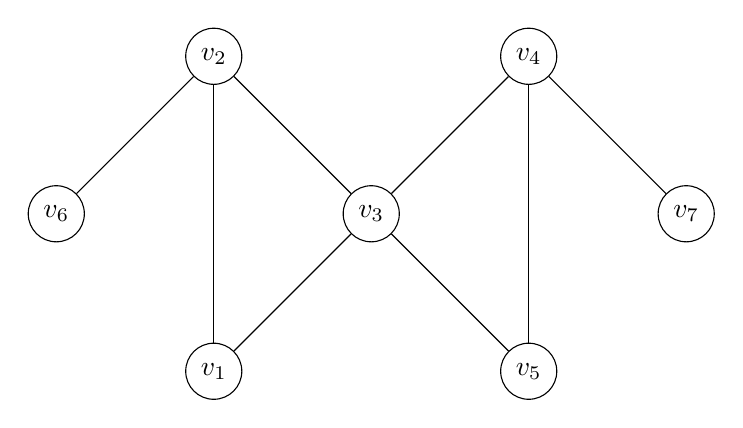
\begin{tikzpicture}[scale =0.5]
	\tikzstyle{every node} = [circle, draw = black]
\node[scale = 1] (0) at (0, 0) {$v_3$};
\node[scale = 1] (1) at (4, -4) {$v_5$};
\node[scale = 1] (2) at (4, 4) {$v_4$};
\node[scale = 1] (3) at (-4, 4) {$v_2$};
\node[scale = 1] (4) at (-4, -4) {$v_1$};
\node[scale = 1] (5) at (-8, 0) {$v_6$};
\node[scale = 1] (6) at (8, 0) {$v_7$};
	\path[draw] (0) -- (1);
	\path[draw] (0) -- (2);
	\path[draw] (0) -- (3);
	\path[draw] (0) -- (4);
	\path[draw] (1) -- (2);
    \path[draw] (4) -- (3);
    \path[draw] (3) -- (5);
    \path[draw] (2) -- (6);
	\end{tikzpicture}
	\caption{Đồ thị vô hướng}\label{fig5}
\end{figure}
\begin{itemize}
    \item Đường đi: $(v_6, v_2, v_1, v_3, v_5, v_4, v_7)$.
    \item Đường đi đơn giản: $(v_7, v_4, v_3, v_5)$.
    \item Chu trình: $(v_1, v_2, v_3, v_1)$.
\end{itemize}  
\end{example}
\begin{definition}
Một đồ thị $G$ liên thông nếu mọi cặp đỉnh bất kỳ của $V$ đều được kết nối bởi một đường đi đơn giản.
\end{definition}
\begin{example}
Đồ thị liên thông và không liên thông được cho bởi Hình 1.6:
\begin{figure}[hpt!]
	\centering
	\begin{tikzpicture}[scale =0.5]
	\tikzstyle{every node} = [circle, draw = black]
\node[scale = 1] (0) at (-16, 0) {$v_3$};
\node[scale = 1] (1) at (-12, -4) {$v_5$};
\node[scale = 1] (2) at (-12, 4) {$v_4$};
\node[scale = 1] (3) at (-20, 4) {$v_2$};
\node[scale = 1] (4) at (-20, -4) {$v_1$};
\node[scale = 1] (5) at (-24, 0) {$v_6$};
\node[scale = 1] (6) at (-8, 0) {$v_7$};
	\path[draw] (0) -- (1);
	\path[draw] (0) -- (2);
	\path[draw] (0) -- (3);
	\path[draw] (0) -- (4);
	\path[draw] (1) -- (2);
    \path[draw] (4) -- (3);
    \path[draw] (3) -- (5);
    \path[draw] (2) -- (6);
\node[scale = 1] (0) at (0, 0) {$v_1$};
\node[scale = 1] (2) at (4, 4) {$v_3$};
\node[scale = 1] (3) at (-4, 4) {$v_4$};
\node[scale = 1] (4) at (-4, -4) {$v_5$};
	\path[draw] (0) -- (2);
	\path[draw] (0) -- (3);
	\path[draw] (2) -- (3);
	\node[scale = 1, draw = none]  at (-0.5,-6)  {(b) Đồ thị không liên thông};
\node[scale = 1, draw = none]  at (-16,-6)  {(a) Đồ thị liên thông};
	\end{tikzpicture}
\caption{Đồ thị liên thông và không liên thông}\label{fig6}
\end{figure}
\end{example}

\begin{definition}
Cho đồ thị $G = (V, E)$, với mỗi cạnh $e = [v_i, v_j] \in E$, hàm $l$ được xác định như sau:
\[
l : E \to \mathbb{R}^+
\]
\[e \mapsto l(e) = l_{ij}\]
Đồ thị $G$ cùng hàm $l$ được gọi là đồ thị có trọng số, ký hiệu là $(G,l)$. Trọng số có thể là độ dài khoảng cách, thời gian, chi phí, lợi nhuận,...
\end{definition}

\begin{example}
Cho đồ thị có trọng số $(G,l)$ như trong Hình 1.7: 
\begin{figure}[hpt!]
	\centering
	\begin{tikzpicture}
	\tikzstyle{every node} = [circle, draw = black]
\node[scale = 1] (0) at (0, 0) {$v_1$};
\node[scale = 1] (1) at (4, -4) {$v_2$};
\node[scale = 1] (2) at (4, 4) {$v_3$};
\node[scale = 1] (3) at (-4, 4) {$v_4$};
\node[scale = 1] (4) at (-4, -4) {$v_5$};

	\path[draw] (0) -- (1);
	\path[draw] (0) -- (2);
	\path[draw] (0) -- (3);
	\path[draw] (0) -- (4);
	\path[draw] (1) -- (2);
    \path[draw] (2) -- (3);
    \path[draw] (3) -- (4);
    \path[draw] (1) -- (4);
    \node[scale = 1, draw = none]  at (-4.5,0)  {$5$};
    \node[scale = 1, draw = none]  at (4.5,0)  {$2$};
	\node[scale = 1, draw = none]  at (0,4.5)  {$4$};
    \node[scale = 1, draw = none]  at (0,-4.5)  {$10$};   
	\node[scale = 1, draw = none]  at (-1.8,2.3)  {$6$};
    \node[scale = 1, draw = none]  at (1.8,2.3)  {$1$};      
     \node[scale = 1, draw = none]  at (-1.8,-2.3)  {$7$};
     \node[scale = 1, draw = none]  at (1.9,-2.3)  {$9$};
	\end{tikzpicture}
	\caption{Đồ thị có trọng số}\label{fig7}
\end{figure}
\end{example}

\section{Đồ thị cây}
\begin{definition}
Cây (tree) $T = (V, E)$ là một đồ thị vô hướng liên thông, không có chu trình. Một đỉnh $v$ thuộc tập đỉnh $V$ của cây $T = (V, E)$ với $\text{deg}(v) = 1$ được gọi là lá.
\end{definition}
\begin{example}
Hình 1.8 là một ví dụ của đồ thị cây.
\begin{figure}[hpt!]
	\centering
	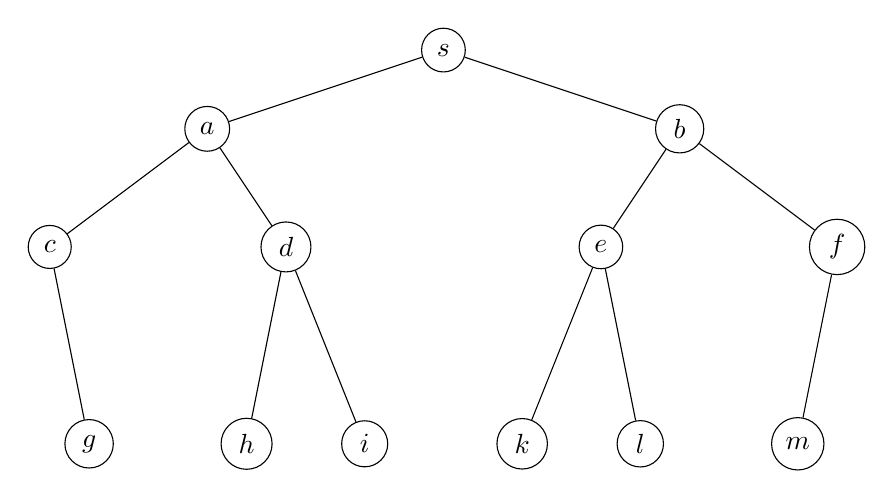
\begin{tikzpicture}[scale =0.5]
	\tikzstyle{every node} = [circle, draw = black]
\node[scale = 1] (0) at (0, 0) {$s$};
\node[scale = 1] (1) at (-6, -2) {$a$};
\node[scale = 1] (2) at (6, -2) {$b$};
\node[scale = 1] (3) at (-10, -5) {$c$};
\node[scale = 1] (4) at (-4, -5) {$d$};
\node[scale = 1] (5) at (4, -5) {$e$};
\node[scale = 1] (6) at (10, -5) {$f$};
\node[scale = 1] (7) at (-9, -10) {$g$};
\node[scale = 1] (8) at (-5, -10) {$h$};
\node[scale = 1] (9) at (-2, -10) {$i$};
\node[scale = 1] (10) at (2, -10) {$k$};
\node[scale = 1] (11) at (5, -10) {$l$};
\node[scale = 1] (12) at (9, -10) {$m$};
	\path[draw] (0) -- (1);
	\path[draw] (0) -- (2);
	\path[draw] (1) -- (3);
	\path[draw] (1) -- (4);
		\path[draw] (2) -- (5);
	\path[draw] (2) -- (6);
 \path[draw] (3) -- (7);
	\path[draw] (4) -- (8);
 \path[draw] (4) -- (9);
	\path[draw] (5) -- (10);
 \path[draw] (5) -- (11);
	\path[draw] (6) -- (12);
 	\end{tikzpicture}
	\caption{Đồ thị cây $T=(V,E)$}\label{fig8}
\end{figure}

Các tính chất của cây:
\begin{itemize}
\item Đồ thị cây có một đỉnh được chọn làm đỉnh gốc, và từ đỉnh gốc này, ta có thể đi tới bất kỳ đỉnh nào khác trong đồ thị cây.
    \item Trong một cây, hai đỉnh bất kỳ được nối với nhau bằng một đường đi sơ cấp duy nhất.
    \item Nếu $T$ là một cây, thì $|E| = |V| - 1$.
    \item Một cạnh $(u, v)$ của $T$ là cạnh cắt khi và chỉ khi $u$ và $v$ không thuộc vào bất cứ chu trình sơ cấp nào của $T$.
    \item Một đồ thị liên thông là một cây khi và chỉ khi mọi cạnh đều là cạnh cắt.
    \item Cho $T$ là một cây bao trùm của đồ thị liên thông $G$ và cho $(u, v)$ là cạnh của $G$ mà không nằm trong $T$. Khi đó, đường đi từ $u$ đến $v$ chứa một chu trình sơ cấp duy nhất.
    \item Một đỉnh $v$ của cây $T$ là một đỉnh cắt của $G$ khi và chỉ khi không tồn tại đỉnh $u \neq v$ sao cho đường đi từ $u$ đến $v$ trong $T$ là đường đi sơ cấp.
    \item Nếu $e$ là cạnh của $T$, thì $T - e$ (đồ thị thu được bằng cách loại bỏ cạnh $e$ khỏi $T$) không còn là cây.
    \item Đồ thị liên thông $G$ có thể được chia thành các cây con nếu và chỉ nếu không có chu trình trong $G$.
\end{itemize}
\end{example}
\section{Bài toán đường đi ngắn nhất trên đồ thị}
Bài toán đường đi ngắn nhất có nhiều ứng dụng trong thực tế, bao gồm hệ thống định tuyến trong mạng lưới, quản lý đường bay của máy bay, tối ưu hóa đường đi trong bản đồ và nhiều lĩnh vực khác.
\begin{definition}
Cho đồ thị $G = (V, E)$, trong đó $V$ là tập hợp các đỉnh và $E$ là tập hợp các cạnh. Một đỉnh xuất phát từ $s$ và một đỉnh đích là $t$.
Bài toán đường đi ngắn nhất trên đồ thị là tìm đường đi từ một đỉnh $s$ đến một đỉnh $t$ sao cho tổng trọng số (hoặc chi phí) của các cạnh trên đường đi là ngắn nhất. 
\end{definition}

Có nhiều thuật toán để giải quyết bài toán này, trong đó ba thuật toán phổ biến nhất là:

\begin{itemize}
    \item \textbf{Thuật toán Dijkstra}: Sử dụng để tìm đường đi ngắn nhất trên đồ thị không có trọng số âm. Thuật toán này duyệt qua các đỉnh xung quanh một cách tương quan để tìm đường đi ngắn nhất từ đỉnh xuất phát đến tất cả các đỉnh khác.
    
    Thuật toán Dijkstra tìm đường đi ngắn nhất trên đồ thị.
\begin{algorithm}[H]
\caption{Thuật toán Dijkstra tìm đường đi ngắn nhất trên đồ thị}
\textbf{Input: } {Đồ thị $G$, đỉnh bắt đầu $s$}

\textbf{Output: } {Khoảng cách ngắn nhất từ $s$ đến tất cả các đỉnh trong $G$}
\begin{algorithmic}
\State \textbf{  for } {mỗi đỉnh $v$ trong $G$} \textbf{do} 
\State\text{               } $   d[v] \leftarrow \infty$;\
\State \text{               }$   visited[v] \leftarrow$ False;\
    \State $d[s] \leftarrow 0$;\
\While{còn đỉnh chưa duyệt}
    \State Chọn một đỉnh $u$ chưa được duyệt có $d[u]$ nhỏ nhất;
    \State \text{               }$   visited[v] \leftarrow$ True;\
        \State \textbf{for} {mỗi đỉnh $v$ kề với $u$} \textbf{do}
        \If{$visited[v]$ và $d[u] + \textit{weight}(u, v) < d[v]$}
            \State $d[v] \leftarrow d[u] + \textit{weight}(u, v)$;
        \EndIf
\EndWhile
\State\textbf{End}
\end{algorithmic}
\end{algorithm}

\begin{example}
Cho đồ thị có trọng số $G=(V,E)$ như trong Hình 1.9. Tìm đường đi ngắn nhất từ đỉnh $s$ đến đỉnh $h$.
\begin{figure}[hpt!]
	\centering
	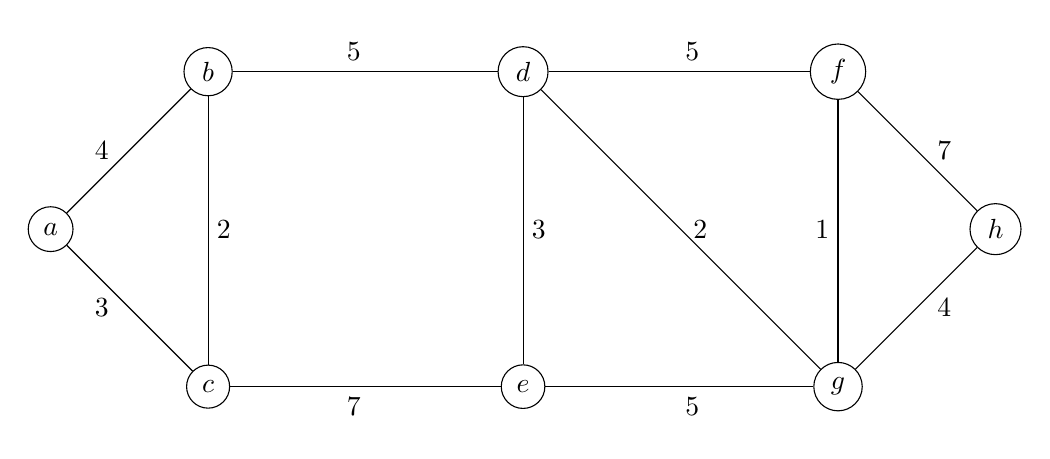
\begin{tikzpicture}[scale =0.5]
	\tikzstyle{every node} = [circle, draw = black]

\node[scale = 1] (1) at (0, -4) {$e$};
\node[scale = 1] (2) at (0, 4) {$d$};
\node[scale = 1] (3) at (8, -4) {$g$};
\node[scale = 1] (4) at (8, 4) {$f$};
\node[scale = 1] (5) at (-8, 4) {$b$};
\node[scale = 1] (6) at (-8, -4) {$c$};
\node[scale = 1] (7) at (-12, 0) {$a$};
\node[scale = 1] (8) at (12, 0) {$h$};

	\path[draw] (7) -- (5);
	\path[draw] (7) -- (6);
	\path[draw] (5) -- (2);
	\path[draw] (1) -- (6);
	\path[draw] (1) -- (2);
    \path[draw] (2) -- (3);
    \path[draw] (3) -- (4);
    \path[draw] (1) -- (3);
    \path[draw] (5) -- (6);
    \path[draw] (4) -- (8);
    \path[draw] (2) -- (4);
    \path[draw] (8) -- (3);
    \node[scale = 1, draw = none]  at (0.4,0)  {$3$};
    \node[scale = 1, draw = none]  at (-7.6,0)  {$2$};
    \node[scale = 1, draw = none]  at (7.6,0)  {$1$};
    \node[scale = 1, draw = none]  at (4.5,0)  {$2$};
	\node[scale = 1, draw = none]  at (4.3,4.5)  {$5$};
    \node[scale = 1, draw = none]  at (-4.3,4.5)  {$5$};
    \node[scale = 1, draw = none]  at (4.3,-4.5)  {$5$};   
	\node[scale = 1, draw = none]  at (-4.3,-4.5)  {$7$};
    \node[scale = 1, draw = none]  at (10.7,2)  {$7$};   
    \node[scale = 1, draw = none]  at (-10.7,2)  {$4$};   
     \node[scale = 1, draw = none]  at (-10.7,-2)  {$3$};
     \node[scale = 1, draw = none]  at (10.7,-2)  {$4$};
	\end{tikzpicture}
	\caption{Đồ thị có trọng số $G=(V,E)$}\label{fig7}
\end{figure}
\end{example}
Để giải bài toán này, ta dùng Thuật toán Dijkstra như sau:
        
\begin{table}[hpt!]
 \caption{Bảng thuật toán Dijkstra để giải Ví dụ 1.9}
    \label{tab1}
\centering
 \begin{tabular}{c c c c c c c c }
  \hline
  $a$ & $b$ & $c$  & $d$ & $e$ & $f$ & $g$ & $h$   \\
  \hline
$0^*$ & $(\infty,-)$ & $(\infty,-)$  & $(\infty,-)$  & $(\infty,-)$ & $(\infty,-)$ & $(\infty,-)$ & $(\infty,-)$ \\
$-$ & $(4,a)$ & $(3,a)^*$  & $(\infty,-)$  & $(\infty,-)$ & $(\infty,-)$  &  $(\infty,-)$ & $(\infty,-)$ \\
$-$ & $(4,a)^*$ & $-$  & $(\infty,-)$  & $(10,c)$ & $(\infty,-)$ &  $(\infty,-)$ & $(\infty,-)$ \\
$-$ & $-$ & $-$  & $(9,b)^*$  & $(10,c)$ & $(\infty,-)$  &  $(\infty,-)$ & $(\infty,-)$ \\
$-$ & $-$ & $-$  & $-$  & $(10,c)^*$ & $(14,d)$  & $(11,d)$ & $(\infty,-)$ \\
$-$ & $-$ & $-$  & $-$  & $-$ & $(14,d)$ & $(11,d)^*$ & $(\infty,-)$ \\
$-$ & $-$ & $-$  & $-$  & $-$ & $(12,g)^*$ & $-$ & $(15,g)$ \\
$-$ & $-$ & $-$  & $-$  & $-$ & $-$ & $-$ & $(15,g)^*$ \\
$-$ & $-$ & $-$  & $-$  & $-$ & $-$ & $-$ & $-$ \\
 \hline
\end{tabular}
    \end{table}
    
Kết thúc Thuật toán, ta được đường đi ngắn nhất từ đỉnh $s$ đến đỉnh $h$ như sau:
$$\{(a,b),(b,d),(d,g),(g,h)\}.$$
Độ dài đường đi ngắn nhất là $4+5+2+4=15.$
Khi đó ta biểu diễn đường đi ngắn nhất như hình vẽ sau:
\begin{figure}[hpt!]
	\centering
	\begin{tikzpicture}[scale =0.5]
	\tikzstyle{every node} = [circle, draw = black]
\node[scale = 1] (2) at (0, 4) {$d$};
\node[scale = 1] (3) at (8, -4) {$g$};
\node[scale = 1] (5) at (-8, 4) {$b$};
\node[scale = 1] (7) at (-12, 0) {$a$};
\node[scale = 1] (8) at (12, 0) {$h$};
	\path[draw] (7) -- (5);
	 \path[draw] (5) -- (2);
      \path[draw] (2) -- (3);
    \path[draw] (8) -- (3);
 \node[scale = 1, draw = none]  at (-4.3,4.5)  {$5$};
  \node[scale = 1, draw = none]  at (-10.7,2)  {$4$};
    \node[scale = 1, draw = none]  at (4.5,0)  {$2$};
     \node[scale = 1, draw = none]  at (10.7,-2)  {$4$};
	\end{tikzpicture}
	\caption{Đường đi ngắn nhất từ $a$ đến $h$ trên đồ thị}\label{fig7}
\end{figure}

    \item \textbf{Thuật toán Bellman-Ford}: Sử dụng để tìm đường đi ngắn nhất trên đồ thị có trọng số âm. Thuật toán này duyệt qua tất cả các cạnh của đồ thị để tìm đường đi ngắn nhất từ đỉnh xuất phát đến tất cả các đỉnh khác.
    
\begin{algorithm}
\caption{Bellman-Ford Algorithm}
\begin{algorithmic}[1]
\Procedure{BellmanFord}{$G, src$}
    \State $V \gets \text{number of vertices in } G$
    \State $E \gets \text{number of edges in } G$
    \State $distance[1 \ldots V] \gets \infty$
    \State $distance[src] \gets 0$
    
    \For{$i \gets 1$ to $V-1$}
        \For{$\text{each edge }(u, v, w) \text{ in } G$}
            \If{$distance[u] + w < distance[v]$}
                \State $distance[v] \gets distance[u] + w$
            \EndIf
        \EndFor
    \EndFor
    
    \For{$\text{each edge }(u, v, w) \text{ in } G$}
        \If{$distance[u] + w < distance[v]$}
            \State \textbf{print} "Graph contains negative weight cycle"
        \EndIf
    \EndFor
    
    \State \textbf{return} $distance[1 \ldots V]$
\EndProcedure
\end{algorithmic}
\end{algorithm}


\begin{example}
Cho đồ thị có hướng $G=(V,E)$ như hình bên dưới, trọng số được ghi trên mỗi cung. Áp dụng thuật toán Bellman - Ford, tìm đường đi ngắn nhất từ đỉnh $a$ đến đỉnh các đỉnh còn lại của đồ thị $G$. Chỉ ra đường đi ngắn nhất từ $a$ đến $f$.
\begin{figure}[hpt!]
	\centering
	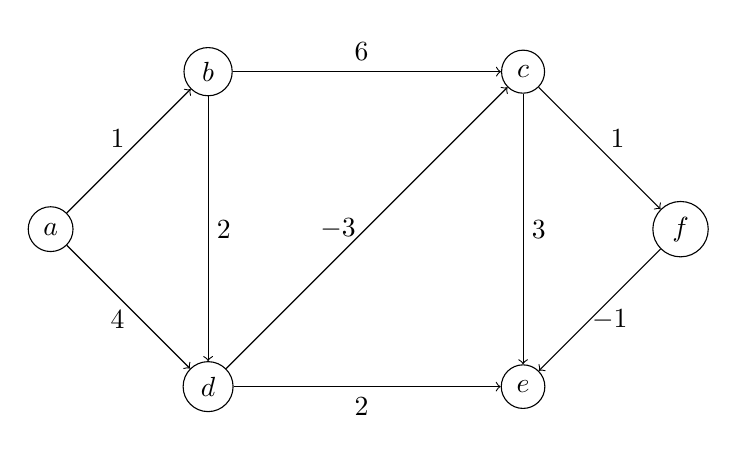
\begin{tikzpicture}[scale =0.5]
	\tikzstyle{every node} = [circle, draw = black]
\node[scale = 1] (1) at (-12, 0) {$a$};
\node[scale = 1] (2) at (-8, 4) {$b$};
\node[scale = 1] (3) at (0, 4) {$c$};
\node[scale = 1] (4) at (-8, -4) {$d$};
\node[scale = 1] (5) at (0, -4) {$e$};
\node[scale = 1] (6) at (4, 0) {$f$};
	\path[draw][->] (1) -- (2);
	\path[draw][->] (2) -- (3);
	\path[draw][->] (1) -- (4);
        \path[draw][->] (3) -- (5);
	\path[draw][->] (6) -- (5);
	\path[draw][->] (2) -- (4);
        \path[draw][->] (4) -- (3);
        \path[draw][->] (4) -- (5);
        \path[draw][->] (3) -- (6);
\node[scale = 1, draw = none]  at (0.4,0) {$3$};
\node[scale = 1, draw = none]  at (-7.6,0){$2$};
\node[scale = 1, draw = none]  at (-4.1,-4.5)  {$2$};
\node[scale = 1, draw = none]  at (-4.1,4.5)  {$6$};
\node[scale = 1, draw = none]  at (-10.3,-2.3)  {$4$};
\node[scale = 1, draw = none]  at (-10.3,2.3)  {$1$};
\node[scale = 1, draw = none]  at (2.2,-2.3)  {$-1$};
\node[scale = 1, draw = none]  at (2.4,2.3)  {$1$};
\node[scale = 1, draw = none]  at (-4.7,0){$-3$};
    \end{tikzpicture}
\caption{Đồ thị $G=(V,E)$}\label{fig7}
\end{figure}

Để giải bài toán này, ta dùng Thuật toán Bellman - Ford như sau:
\begin{table}[hpt!]
        \centering
         \caption{Bảng thuật toán Bellman - Ford để giải Ví dụ 1.10}
        \label{tab1}
       \begin{tabular}{c c c c c c c }
  \hline
  $k$ & $d[a],truoc[a]$ & $d[b],truoc[b]$  & $d[c],truoc[c]$ & $d[d],truoc[d]$ & $d[e],truoc[e]$ & $d[f],truoc[f]$ \\
  \hline
 & $(0,1)$ & $(1,1)$  & $(\infty,1)$  & $(4,1)$ & $(\infty,1)$ & $(\infty,1)$ \\
$1$ & $(0,1)$ & $(1,1)$  & $(1,4)$  & $(3,2)$ & $(4,3)$  &  $(2,3)$ \\
$2$ & $(0,1)$ & $(1,1)$  & $(0,4)$  & $(3,2)$ & $(1,6)$ &  $(1,3)$\\
$3$ & $(0,1)$ & $(1,1)$  & $(0,4)$  & $(3,2)$ & $(0,6)$  &  $(1,3)$  \\
$4$ & $(0,1)$ & $(1,1)$  & $(0,4)$  & $(3,2)$ & $(0,6)$  & $(1,3)$  \\

 \hline
\end{tabular}
    \end{table}
    
Kết thúc Thuật toán, ta được đường đi ngắn nhất từ đỉnh $a$ đến đỉnh $f$ như sau:
$$a \longrightarrow b \longrightarrow d \longrightarrow c \longrightarrow f,$$
với $d[f]=1$.
\clearpage
Khi đó ta biểu diễn đường đi ngắn nhất như hình vẽ sau:
\begin{figure}[hpt!]
	\centering
	\begin{tikzpicture}[scale =0.5]
	\tikzstyle{every node} = [circle, draw = black]
\node[scale = 1] (1) at (-12, 0) {$a$};
\node[scale = 1] (2) at (-8, 4) {$b$};
\node[scale = 1] (3) at (0, 4) {$c$};
\node[scale = 1] (4) at (-8, -4) {$d$};
\node[scale = 1] (6) at (4, 0) {$f$};
	\path[draw][->] (1) -- (2);
	\path[draw][->] (2) -- (4);
        \path[draw][->] (4) -- (3);
        \path[draw][->] (3) -- (6);
\node[scale = 1, draw = none]  at (-7.6,0){$2$};
\node[scale = 1, draw = none]  at (-10.3,2.3)  {$1$};
\node[scale = 1, draw = none]  at (2.4,2.3)  {$1$};
\node[scale = 1, draw = none]  at (-4.7,0){$-3$};
	\end{tikzpicture}
	\caption{Đường đi ngắn nhất từ $a$ đến $f$}\label{fig7}
\end{figure}
\end{example}

\item \textbf{Thuật toán Floyd-Warshall}: Thuật toán  còn được gọi là thuật toán Floyd được Robert Floyd tìm ra năm 1962 là thuật toán để tìm đường đi ngắn nhất giữa mọi cặp đỉnh. Floyd hoạt động được trên đồ thị có hướng, có thể có trọng số âm, tuy nhiên không có chu trình âm. Ngoài ra, Floyd còn có thể được dùng để phát hiện chu trình âm.

Thuật toán Floyd-Warshall tìm đường đi ngắn nhất trên đồ thị.
\end{itemize}

\begin{algorithm}
\caption{Floyd-Warshall Algorithm}
\begin{algorithmic}[1]
\Procedure{FloydWarshall}{$G$}
    \State $V \gets \text{number of vertices in } G$
    \State $distance[1 \ldots V][1 \ldots V] \gets \infty$
    
    \For{$i \gets 1$ to $V$}
        \For{$j \gets 1$ to $V$}
            \If{$i = j$}
                \State $distance[i][j] \gets 0$
            \ElsIf{$(i, j)$ is an edge in $G$}
                \State $distance[i][j] \gets \text{weight of edge } (i, j)$
            \EndIf
        \EndFor
    \EndFor
    
    \For{$k \gets 1$ to $V$}
        \For{$i \gets 1$ to $V$}
            \For{$j \gets 1$ to $V$}
                \If{$distance[i][j] > distance[i][k] + distance[k][j]$}
                    \State $distance[i][j] \gets distance[i][k] + distance[k][j]$
                \EndIf
            \EndFor
        \EndFor
    \EndFor
    
    \State \textbf{return} $distance[1 \ldots V][1 \ldots V]$
\EndProcedure
\end{algorithmic}
\end{algorithm}
\clearpage
\begin{example}
Cho đồ thị vô hướng $G=(V,E)$ như hình vẽ bên dưới. Tìm đường đi ngắn nhất giữa các cặp đỉnh đã cho.
\begin{figure}[hpt!]
	\centering
	\begin{tikzpicture}[scale =0.5]
	\tikzstyle{every node} = [circle, draw = black]
\node[scale = 1] (5) at (0, -4) {$a$};
\node[scale = 1] (4) at (-8, -4) {$b$};
\node[scale = 1] (2) at (-8, 4) {$c$};
\node[scale = 1] (3) at (0, 4) {$d$};
\node[scale = 1] (6) at (4, 0) {$e$};	
	\path[draw] (2) -- (3);
        \path[draw] (3) -- (5);
	\path[draw] (6) -- (5);
	\path[draw] (2) -- (4);
        \path[draw] (4) -- (5);
        \path[draw] (3) -- (6);
\node[scale = 1, draw = none]  at (0.4,0) {$9$};
\node[scale = 1, draw = none]  at (-7.6,0){$2$};
\node[scale = 1, draw = none]  at (-4.1,-4.5)  {$5$};
\node[scale = 1, draw = none]  at (-4.1,4.5)  {$7$};
\node[scale = 1, draw = none]  at (2.2,-2.3)  {$1$};
\node[scale = 1, draw = none]  at (2.4,2.3)  {$2$};
	\end{tikzpicture}
	\caption{Đồ thị vô hướng $G=(V,E)$}\label{fig7}
\end{figure}
\end{example}
Với ví dụ trên, ta mô tả cách thuật toán toán Floyd Warshall như sau:

Khởi tạo ma trận khoảng cách ban đầu, ta được:
\begin{table}[hpt!]
        \centering
      \caption{Bảng Thuật toán Floyd-Warshall}
        \label{tab1}
       \begin{tabular}{ c c c c c c }
  \hline
   & $a$ & $b$  & $c$ & $d$ & $e$  \\
   \hline
$a$ & $0$ & $5$  & $\infty$  & $9$ & $1$\\
$b$ & $5$ & $0$  & $2$  & $\infty$ & $\infty$\\
$c$ & $\infty$ & $2$  & $0$  & $7$ & $\infty$\\
$d$ & $9$ & $\infty$  & $7$  & $0$ & $2$\\
$e$ & $1$ & $\infty$  & $\infty$  & $2$ & $0$\\
 \hline
\end{tabular}
    \end{table}

Quá trình thuật toán diễn ra như sau:

Chọn lần lượt từng đỉnh của đồ thị làm đỉnh trung gian (ta quy ước là $K$). Chọn một cặp 2 đỉnh phân biệt và không trùng với đỉnh trung gian (ta quy ước lần lượt là $I$ và $J$).

Thực hiện so sánh như ở trên: Đường đi ngắn nhất giữa $I$ và $J$ sẽ bằng giá trị nhỏ nhất của một trong hai giá trị sau:
\begin{itemize}
    \item Giá trị đường đi ngắn nhất hiện thời giữa 
$I$ và $J$.
\item Tổng của giá trị đường đi ngắn nhất hiện thời giữa $I$ và $K$ và đường đi ngắn nhất hiện thời giữa $K$ và $J$.
\end{itemize}
Đầu tiên, $K=1$. Nhờ đỉnh $a$ làm trung gian, ta thấy xuất hiện đường đi từ đỉnh $b$ tới đỉnh $d$ (độ dài 14) và từ đỉnh $b$ tới đỉnh $e$ (độ dài 6). Đường đi trung gian qua đỉnh $a$ để đi từ đỉnh $d$ tới đỉnh $e$ không tối ưu về chiều dài $(9+1>2)$ nên ta không cập nhật lại đường đi ngắn nhất giữa hai đỉnh $d$ và $e$.

Mảng lúc này trở thành:
\begin{table}[hpt!]
        \centering
          \caption{Bảng Thuật toán Floyd-Warshall}
        \label{tab1}
       \begin{tabular}{c c c c c c}
  \hline
   & $a$ & $b$  & $c$ & $d$ & $e$  \\
  \hline
$a$ & $0$ & $5$  & $\infty$  & $9$ & $1$\\
$b$ & $5$ & $0$  & $2$  & $14$ & $6$\\
$c$ & $\infty$ & $2$  & $0$  & $7$ & $\infty$\\
$d$ & $9$ & $14$  & $7$  & $0$ & $2$\\
$e$ & $1$ & $6$  & $\infty$  & $2$ & $0$\\
 \hline
\end{tabular}
    \end{table}
    
Tiếp theo, ta duyệt tới $K=2$. Đường đi từ 
$c$ tới $a$ (độ dài 7), từ $c$ tới $e$ (độ dài 8) được hình thành. Đường đi từ $c$ tới 
$d$ không cập nhật độ dài $(7<2+5+9)$.
\begin{table}[hpt!]
        \centering
             \caption{Bảng Thuật toán Floyd-Warshall}
        \label{tab1}
       \begin{tabular}{c c c c c c }
  \hline
   & $a$ & $b$  & $c$ & $d$ & $e$  \\
  \hline
$a$ & $0$ & $5$  & $7$  & $9$ & $1$\\
$b$ & $5$ & $0$  & $2$  & $14$ & $6$\\
$c$ & $7$ & $2$  & $0$  & $7$ & $8$\\
$d$ & $9$ & $14$  & $7$  & $0$ & $2$\\
$e$ & $1$ & $6$  & $8$  & $2$ & $0$\\
 \hline
\end{tabular}
    \end{table}

Cứ tiếp tục lựa chọn $K$ như vậy cho tới hết, ta sẽ thu được mảng 2D hoàn chỉnh:
\clearpage
\begin{table}[hpt!]
        \centering
    \caption{Bảng Thuật toán Floyd-Warshall}
        \label{tab1}
       \begin{tabular}{c c c c c c }
  \hline
   & $a$ & $b$  & $c$ & $d$ & $e$  \\
  \hline
$a$ & $0$ & $5$  & $7$  & $3$ & $1$\\
$b$ & $5$ & $0$  & $2$  & $8$ & $6$\\
$c$ & $7$ & $2$  & $0$  & $7$ & $8$\\
$d$ & $3$ & $8$  & $7$  & $0$ & $2$\\
$e$ & $1$ & $6$  & $8$  & $2$ & $0$\\
 \hline
\end{tabular}
    \end{table}

Giả sử qua mảng này, ta thấy đường đi ngắn nhất từ đỉnh $b$ tới đỉnh $d$ có độ dài 
8. Dựa theo đồ thị thì nó là đoạn đường sau: $b \longrightarrow a \longrightarrow e \longrightarrow d$.
\begin{figure}[hpt!]
	\centering
	\begin{tikzpicture}[scale =0.5]
	\tikzstyle{every node} = [circle, draw = black]
\node[scale = 1] (5) at (0, -4) {$a$};
\node[scale = 1] (4) at (-8, -4) {$b$};
\node[scale = 1] (3) at (0, 4) {$d$};
\node[scale = 1] (6) at (4, 0) {$e$};	
	\path[draw] (6) -- (5);
        \path[draw] (4) -- (5);
        \path[draw] (3) -- (6);
\node[scale = 1, draw = none]  at (-4.1,-4.5)  {$5$};
\node[scale = 1, draw = none]  at (2.2,-2.3)  {$1$};
\node[scale = 1, draw = none]  at (2.4,2.3)  {$2$};
	\end{tikzpicture}
	\caption{Đường đi ngắn nhất giữa các cặp đỉnh đã cho}\label{fig7}
\end{figure}

\section{Bài toán 1-center trên đồ thị}
\begin{definition}
Cho một đồ thị $G = (V, E),$ trong đó $V$ là tập hợp các đỉnh và $E$ là tập hợp các cạnh của đồ thị. Mỗi cạnh $e \in E$ có một độ dài $l_e$. Ta  ký hiệu $d(u,v)$ là khoảng cách giữa hai đỉnh $u$ và $v$ (đường đi ngắn nhất trên $G$ nối hai đỉnh). Khoảng cách từ một điểm bất kỳ $p$ nằm trên cạnh $e \equiv (u,u')$ của $G$ tới $u$ được cho bởi $d(u,p) \equiv \lambda l_e$ với $0 \le \lambda \le 1$. Ta thấy rằng $p \equiv u$ khi $\lambda =0$ và $p \equiv u'$ khi $\lambda =1$. Gọi $P(G)$ là tập hợp tất cả các điểm trên $G$. Bài toán 1-center (absolute 1-center) là tìm một điểm $p$ thuộc $P(G)$ sao cho tối thiểu hàm mục tiêu center sau
\begin{align}
    \max \sum\limits_{v \in V} {d(p,v)} 
\end{align}
Điểm $p$ thỏa mãn bài toán trên được gọi là điểm (absolute) 1-center của $G$.
\end{definition}
Thuật toán tìm 1-center trên cây đồ thị
\begin{algorithm}[H]
\caption{Thuật toán tìm 1-center trên cây đồ thị}
\textbf{Input:} Cây $T$ và hàm cạnh $l$

\textbf{Output:} $X^*(T)$
\begin{algorithmic}
\State \textbf{Begin}
\State Chọn $x \in P(T)$;
\State Xác định $v \in V$ với $d(x,v)=\underset{i\in M}{\mathop{\max }}\,d\left( x,{{v}_{i}} \right)$;
\State Xác định $w \in V$ với $d(v,w)=\underset{i\in M}{\mathop{\max }}\,d\left( x,{{w}_{i}} \right)$;
\State Output $X^*(T)=x^*$ với $d(x^*,v)=d(x^*,w)=\frac{1}{2}d(v,w)$;
\State \textbf{End} 
\end{algorithmic}
\end{algorithm}
\begin{example}
Cho đồ thị cây $T=(V,E)$ như trong Hình 1.15. Tìm điểm $x^*$ là 1-center của đồ thị cây $T$. 
\begin{figure}[hpt!]
	\centering
	\begin{tikzpicture}[scale =0.5]
	\tikzstyle{every node} = [circle, draw = black]
\node[scale = 1] (1) at (0, 0) {$v_1$};
\node[scale = 1] (2) at (0, -4) {$v_2$};
\node[scale = 1] (3) at (-4, -8) {$v_3$};
\node[scale = 1] (4) at (4, -8) {$v_4$};
\node[scale = 1] (5) at (0, -12) {$v_5$};
\node[scale = 1] (6) at (8, -12) {$v_6$};

	\path[draw] (1) -- (2);
	\path[draw] (2) -- (3);
	\path[draw] (2) -- (4);
	\path[draw] (4) -- (6);
	\path[draw] (4) -- (5);
\node[scale = 1, draw = none]  at (0.5,-2)  {$1$};
\node[scale = 1, draw = none]  at (-2.7,-6)  {$2$};
\node[scale = 1, draw = none]  at (2.7,-6)  {$6$};
\node[scale = 1, draw = none]  at (2.7,-10)  {$5$};
\node[scale = 1, draw = none]  at (6.7,-10)  {$4$};
	\end{tikzpicture}
	\caption{Đồ thị cây $T=(V,E)$}\label{fig7}
\end{figure}
\end{example}
Áp dụng Thuật toán trên ta được:
\begin{itemize}
    \item $x=v_4$
    \item ${v=v_3}$
    \item ${w=v_5}$
    \item $x^*=(\{v_2,v_4,\frac{3}{4}\})$
\end{itemize}
Ta được $g^*(x^*)=6.5.$
 \chapter{BÀI TOÁN NGƯỢC 1-CENTER NHANH NHẤT TRÊN CÂY}
 Ở chương này tập trung vào bài toán ngược 1-center trên cây và bao gồm hai phần chính. Phần đầu tiên giới thiệu các kí hiệu và định nghĩa cơ bản liên quan đến bài toán, giúp định rõ khung làm việc. Phần thứ hai trình bày một số tính chất quan trọng của điểm 1-center nhanh nhất tuyệt đối, tập trung vào cách tối ưu hóa vị trí của điểm này trong cây và tác động của nó đối với bài toán. Chương này cung cấp một cơ sở lý thuyết quan trọng cho việc nghiên cứu và giải quyết bài toán ngược 1-center trên cây.
 \section{Kí hiệu và định nghĩa}
\hspace*{0.3cm}
	Cho $T=\left( V,E \right)$ là cây vô hướng bởi tập $V$ gồm $n$ đỉnh và tập $E$ gồm $m=n-1$ cạnh. Ta biểu thị một cạnh từ đỉnh $i$ đến đỉnh $j$ bởi $\left( i,j \right)\in E$ có hai tham số liên quan: trọng tải (capacity) $c\left( i,j \right)\ge 0,$ biểu thị mức tối đa khả năng có thể di chuyển trên cạnh và thời gian đi qua (lead time) $l\left( i,j \right)\ge 0$ biểu thị thời gian cần thiết để đi qua cạnh. Đặt $t$ là một đỉnh phân biệt trong cây, một đường đi vô hướng $P$ (undirected path) từ đỉnh $i\in V$ đến đỉnh $t$ là một chuỗi $i={{i}_{1}},{{i}_{2}},...,{{i}_{k}}=t$ khác các đỉnh của $V$ sao cho $\left( {{i}_{r}},{{i}_{r+1}} \right)\in E$ với $r=1,2,...,k-1.$ 

 
Đặt \begin{equation}
l\left( P \right)=\sum\limits_{\left( i,j \right)\in P}{l\left( i,j \right)}
\end{equation}
là thời gian đi qua $P$ và 
\begin{equation}
c\left( P \right) = \mathop {\min }\limits_{\left( {i,j} \right) \in P} {\mkern 1mu} c\left( {i,j} \right)
\end{equation}
là trọng tải của $P.$ 

Cho hai đỉnh $s,\,t$ và giá trị $\sigma $ cho trước. Thời gian truyền (transmission time) của đường dẫn $P:\left( s={{v}_{1}},{{v}_{2}},...,{{v}_{k}}=t \right)$ để gửi $\sigma $ đơn vị dữ liệu từ $s$ đến $t$ được xác định như sau:
\begin{equation}
T\left( P,t,\sigma  \right)=l\left( P \right)+\frac{\sigma }{c\left( P \right)}.  
\end{equation}

Đặt ${{P}_{st}}$ là tập hợp các đường đi giữa các đỉnh $s$ và $t.$ Thời gian truyền tối thiếu để gửi $\sigma $ đơn vị dữ liệu từ đỉnh $s$ đến $t$ được xác định như sau:
$$Q\left( s,t,\sigma  \right)=\underset{P\in {{P}_{st}}}{\mathop{\min }}\,\left\{ T\left( P,t,\sigma  \right) \right\}.$$

Đường dẫn $P^*$ từ đỉnh $s$ đến $t$ được gọi là đường dẫn nhanh nhất từ $s$ đến $t$ nếu $Q\left( s,t,\sigma  \right)=T\left( P^*,t,\sigma  \right).$

\begin{example}
Cho cây $T=(V,E)$ như hình bên dưới với $\sigma =10$.
\begin{figure}[H]
	\centering
	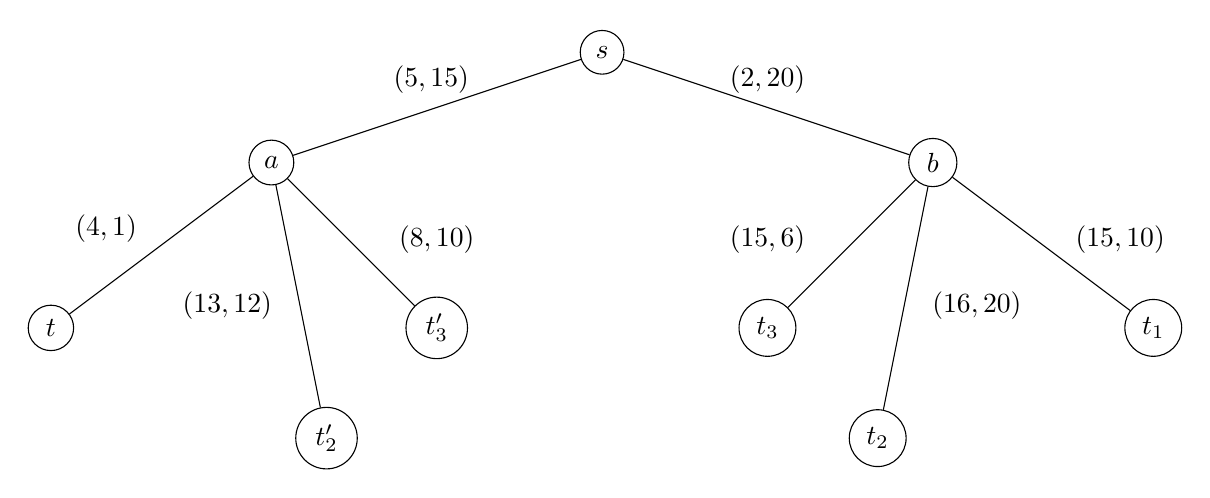
\begin{tikzpicture}[scale =0.7]
	\tikzstyle{every node} = [circle, draw = black]
\node[scale = 1] (0) at (0, 0) {$s$};
\node[scale = 1] (1) at (-6, -2) {$a$};
\node[scale = 1] (2) at (6, -2) {$b$};
\node[scale = 1] (3) at (-10, -5) {$t$};
\node[scale = 1] (4) at (-5, -7) {$t'_2$};
\node[scale = 1] (5) at (5, -7) {$t_2$};
\node[scale = 1] (6) at (10, -5) {$t_1$};
\node[scale = 1] (7) at (-3, -5) {$t'_3$};
\node[scale = 1] (8) at (3, -5) {$t_3$};
    
	\node[scale = 1, draw = none]  at (-3.1,-0.5)  {$(5,15)$};
    \node[scale = 1, draw = none]  at (3,-0.5)  {$(2,20)$};
	\node[scale = 1, draw = none]  at (-9,-3.2)  {$(4,1)$};
    \node[scale = 1, draw = none]  at (9.4,-3.4)  {$(15,10)$};   
	\node[scale = 1, draw = none]  at (-6.8,-4.6)  {$(13,12)$};
    \node[scale = 1, draw = none]  at (6.8,-4.6)  {$(16,20)$};      
     \node[scale = 1, draw = none]  at (-3,-3.4)  {$(8,10)$};
     \node[scale = 1, draw = none]  at (3,-3.4)  {$(15,6)$};
	\path[draw] (0) -- (1);
	\path[draw] (0) -- (2);
	\path[draw] (1) -- (3);
	\path[draw] (1) -- (4);
	%\path[draw] (1) -- (6);
	\path[draw] (2) -- (5);
	\path[draw] (2) -- (6);
 \path[draw] (1) -- (7);
	\path[draw] (2) -- (8);
	\end{tikzpicture}
	\caption{Cây $T=(V,E)$}\label{fig12}
\end{figure}


Ta xét đường đi ${{P}_{st}}$ thì các giá trị
$l(P)$, $c(P)$, $T(P,t,\sigma)$ như sau:
\begin{itemize}
\item $l(P)=5+4=9.$
\item $c(P)=\min\{1,15\}=1.$
\item $T\left( P,t,\sigma  \right)=9+\frac{10}{1}=19.$
\end{itemize}

\end{example}
\begin{example}
Ta chọn $\sigma=12$. Xét đồ thị $G$ sau:
\begin{figure}[hpt!]
	\centering
	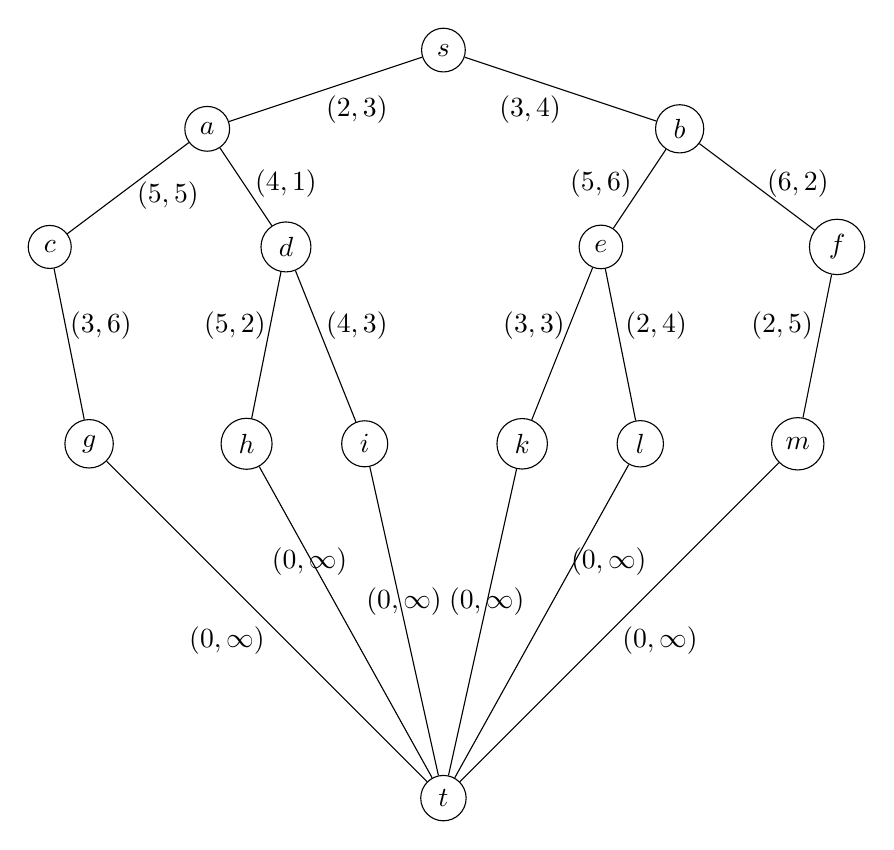
\begin{tikzpicture}[scale =0.5]
	\tikzstyle{every node} = [circle, draw = black]
\node[scale = 1] (0) at (0, 0) {$s$};
\node[scale = 1] (1) at (-6, -2) {$a$};
\node[scale = 1] (2) at (6, -2) {$b$};
\node[scale = 1] (3) at (-10, -5) {$c$};
\node[scale = 1] (4) at (-4, -5) {$d$};
\node[scale = 1] (5) at (4, -5) {$e$};
\node[scale = 1] (6) at (10, -5) {$f$};
\node[scale = 1] (7) at (-9, -10) {$g$};
\node[scale = 1] (8) at (-5, -10) {$h$};
\node[scale = 1] (9) at (-2, -10) {$i$};
\node[scale = 1] (10) at (2, -10) {$k$};
\node[scale = 1] (11) at (5, -10) {$l$};
\node[scale = 1] (12) at (9, -10) {$m$};
\node[scale = 1] (13) at (0, -19) {$t$};
	\node[scale = 1, draw = none]  at (-2.2,-1.5)  {$(2,3)$};
    \node[scale = 1, draw = none]  at (2.2,-1.5)  {$(3,4)$};
	\node[scale = 1, draw = none]  at (-7,-3.7)  {$(5,5)$};
        \node[scale = 1, draw = none]  at (9,-3.4)  {$(6,2)$};
	\node[scale = 1, draw = none]  at (-4,-3.4)  {$(4,1)$};
        \node[scale = 1, draw = none]  at (4,-3.4)  {$(5,6)$};
        
     \node[scale = 1, draw = none]  at (2.3,-7)  {$(3,3)$};
     \node[scale = 1, draw = none]  at (5.4,-7)  {$(2,4)$};
      \node[scale = 1, draw = none]  at (8.6,-7)  {$(2,5)$};
     \node[scale = 1, draw = none]  at (-2.2,-7)  {$(4,3)$};
      \node[scale = 1, draw = none]  at (-5.3,-7)  {$(5,2)$};
     \node[scale = 1, draw = none]  at (-8.7,-7)  {$(3,6)$}; 
     
     \node[scale = 1, draw = none]  at (-5.5,-15)  {$(0,\infty)$};
     \node[scale = 1, draw = none]  at (-3.4,-13)  {$(0,\infty)$};
      \node[scale = 1, draw = none]  at (-1,-14)  {$(0,\infty)$};
     \node[scale = 1, draw = none]  at (1.1,-14)  {$(0,\infty)$};
      \node[scale = 1, draw = none]  at (4.2,-13)  {$(0,\infty)$};
     \node[scale = 1, draw = none]  at (5.5,-15)  {$(0,\infty)$};
     
	\path[draw] (0) -- (1);
	\path[draw] (0) -- (2);
	\path[draw] (1) -- (3);
	\path[draw] (1) -- (4);
		\path[draw] (2) -- (5);
	\path[draw] (2) -- (6);
 \path[draw] (3) -- (7);
	\path[draw] (4) -- (8);
 \path[draw] (4) -- (9);
	\path[draw] (5) -- (10);
 \path[draw] (5) -- (11);
	\path[draw] (6) -- (12);
 \path[draw] (7) -- (13);
 \path[draw] (8) -- (13);
 \path[draw] (9) -- (13);
 \path[draw] (10) -- (13);
 \path[draw] (11) -- (13);
 \path[draw] (12) -- (13);
	\end{tikzpicture}
	\caption{Đồ thị $G=(V,E)$}\label{fig9}
\end{figure}

Ta xét đường đi ${{P}_{sg}}$ thì các giá trị
$l(P)$, $c(P)$, $T(P,t,\sigma)$ như sau:
\begin{itemize}
\item $l(P)=2+5+3=10.$
\item $c(P)=\min\{3,5,6\}=3.$
\item $T\left( P,t,\sigma  \right)=10+\frac{12}{3}=14.$
\end{itemize}
Tương tự ta có bảng giá trị như sau:
    \begin{table}[H]
        \centering
\caption{Bảng tính thời gian, trọng tải và thời gian truyền với $\sigma =12$}
        \label{tab1}
       \begin{tabular}{c c c c }
  \hline
  Đường đi & $l(P)$ & $c(P)$  & $T(P,t,\sigma )$   \\
  \hline
${{P}_{sh}}$ & $11$    & $1$  & $23$\\
${{P}_{si}}$ & $10$    & $1$  & $22$ \\
${{P}_{sk}}$ & $11$    & $3$  & $15$ \\
${{P}_{sl}}$ & $10$    & $4$  & $13$ \\
${{P}_{sm}}$ & $11$    & $2$  & $17$ \\
 \hline
\end{tabular}
    \end{table}
Khi đó: $Q\left( s,t,\sigma  \right)=13.$
\end{example}
\begin{remark}
    Trong mỗi cây, giữa hai đỉnh $s,t\in V$ luôn tồn tại một đường đi duy nhất $P,$ nghĩa là ${{P}_{st}}=\left\{ P \right\}$ và $Q\left( s,t,\sigma  \right)=T\left( P,t,\sigma  \right).$
\end{remark}
\begin{definition}
    Cho đồ thị cây $T$ và giá trị $\sigma $ cho trước. Bài toán vị trí 1-center nhanh nhất tuyệt đối (absolute quickest 1-center) của đồ thị cây $T$ là bất kì đỉnh $s^*$ nào được đặt trên các đỉnh hoặc các cạnh của đồ thị cây $T$ với đặc tính là thời gian truyền để gửi $\sigma $ đơn vị dữ liệu từ đỉnh xa nhất tới $s^*$ là giá trị nhỏ nhất. Bài toán vị trí 1-center nhanh nhất trên cây $T$ có thể được viết dưới dạng sau:
$$\underset{s\in T}{\mathop{\min }}\,\underset{t\in V}{\mathop{\max }}\,\left\{ Q\left( s,t,\sigma  \right) \right\}.$$
\end{definition}

\begin{definition}
Cho đồ thị cây $T$, giá trị $\sigma $ và đỉnh $s^*$ cho trước. Bài toán ngược 1-center nhanh nhất tuyệt đối (inverse absolute quickest 1-center location problem) của đồ thị cây $T$ làm thay đổi trọng tải với tổng chi phí tối thiểu sao cho $s^*$ thành vị trí 1-center nhanh nhất. Để thuận tiện, ta nói bài toán ngược 1-center nhanh nhất trên cây thay vì bài toán vị trí ngược 1-center nhanh nhất tuyệt đối trên cây.
\end{definition}





 \kl 
\begin{itemize}
\item Luận văn này đã xem xét bài toán ngược 1-center nhanh nhất trên cây với biến là trọng tải cạnh. Hai dạng bài toán được xem xét là giảm trọng tải cạnh và tăng trọng tải cạnh điều được giải quyết trong thời gian tuyến tính. 
\item Trong tương lai, hướng nghiên cứu mở rộng của đề tài này là giải quyết các bài toán liên quan đến lý thuyết vị trí có yếu tố "nhanh nhất", đặc biệt là bài toán ngược.
\end{itemize}
\newpage
\begin{thebibliography}{99}
	\bibitem{1} R. Ahuja, T. Magnanti, J. Orlin, \emph{Network Flows: Theory, Algorithms, and Applications}, Prentice Hall, 1993.
    \bibitem{2} B. Alizadeh, R.E. Burkard, \emph{Combinatorial algorithms for inverse absolute and vertex 1-center location problems on trees}, \emph{Networks} 58 (3) (2011) 190–200.
    \bibitem{3} B. Alizadeh, R.E. Burkard, \emph{A linear time algorithm for inverse obnoxious center location problems on networks}, \emph{CEJOR Cent. Eur. J. Oper. Res.} 21 (2013) 585–594.
    \bibitem{4} B. Alizadeh, R.E. Burkard, U. Pferschy, \emph{Inverse 1-center location problems with edge length augmentation on trees}, \emph{Computing} 86 (2009) 331–343.
    \bibitem{5} B. Alizadeh, R. Etemad, \emph{The linear time optimal approaches for reverse obnoxious center location problems on networks}, \emph{Optimization} 65 (2016) 2025–2036.
    \bibitem{6} F.B. Bonab, R.E. Burkard, E. Gassner, \emph{Inverse p-median problems with variable edge lengths}, \emph{Math. Methods Oper. Res.} 73 (2011) 263–280.
    \bibitem{7} R.E. Burkard, H. Dollani, \emph{A note on the robust 1-center problem on trees}, \emph{Ann. Oper. Res.} 110 (2002) 69–82.
    \bibitem{8} R.E. Burkard, J. Fathali, \emph{A polynomial method for the pos/neg weighted 3-median problem on a tree}, \emph{Math. Methods Oper. Res.} 65 (2007) 229–238.
    \bibitem{9} R.E. Burkard, J. Fathali, H.T. Kakhki, \emph{The p-maxian problem on a tree}, \emph{Oper. Res. Lett.} 35 (2007) 331–335.
    \bibitem{10} R.E. Burkard, M. Galavii, E. Gassner, \emph{The inverse Fermat-Weber problem}, \emph{European J. Oper. Res.} 206 (2010) 11–17.
    \bibitem{11} R.E. Burkard, J. Hatzl, \emph{Median problems with positive and negative weights on cycles and cacti}, \emph{J. Comb. Optim.} 20 (2010) 27–46.
    \bibitem{12} R.E. Burkard, C. Pleschiutschnig, J. Zhang, \emph{Inverse median problems}, \emph{Discrete Optim.} 1 (1) (2004) 23–39.
    \bibitem{13} R.E. Burkard, C. Pleschiutschnig, J. Zhang, \emph{The inverse 1-median problem on a cycle}, \emph{Discrete Optim.} 5 (2) (2008) 242–253.
    \bibitem{14} M.C. Cai, X.G. Yang, J.Z. Zhang, \emph{The complexity analysis of the inverse center location problem}, \emph{J. Global Optim.} 15 (2) (1999) 213–218.
    \bibitem{15} H.I. Calvete, L. del Pozo, J.A. Iranzo, \emph{Algorithms for the quickest path problem and the reliable quickest path problem}, \emph{Comput. Manag. Sci.} 9 (2012) 255–272.
    \bibitem{16} Y. Chen, Y. Chin, \emph{The quickest path problem}, \emph{Comput. Oper. Res.} 17 (2) (1990) 153–161.
    \bibitem{17} M.S. Daskin, \emph{Network and Discrete Location: Models, Algorithms, and Applications}, John Wiley Sons, 2011.
    \bibitem{18} R. Etemad, B. Alizade, \emph{Reverse selective obnoxious center location problems on tree graphs}, \emph{Math. Methods Oper. Res.} 87 (2018) 431–450.
    \bibitem{19} M. Galavii, \emph{Inverse 1-median problems}, Ph.D. Disseration, Graz University of Technology, 2008.
    \bibitem{20} Gassner, \emph{The inverse 1-maxian problem with edge length modification}, \emph{J. Comb. Optim.} 16 (1) (2008) 50–67.
    \bibitem{21} E. Gassner, \emph{An inverse approach to convex ordered median problems in trees}, \emph{J. Comb. Optim.} 23 (2) (2012) 261–273.
    \bibitem{22} X. Guan, B. Zhang, \emph{Inverse 1-median problem on trees under weighted Hamming distance}, \emph{J. Global Optim.} 54 (1) (2012) 75–82.
    \bibitem{23} H.W. Hamacher, Z. Drezner, \emph{Facility Location: Applications and Theory}, Springer Science and Business Media, 2002.
    \bibitem{24} C. Heuberger, \emph{Inverse combinatorial optimization: A survey on problems, methods, and results}, \emph{J. Comb. Optim.} 8 (3) (2004) 329–361.
    \bibitem{25} Y.C. Hung, G.H. Chen, \emph{Distributed algorithms for the quickest path problem}, \emph{Parallel Comput.} 18 (1992) 823–834.
    \bibitem{26} G. Laporte, S. Nickel, F.S. da Gama, \emph{Introduction to Location Science in Location Science}, Springer, 2015, pp. 1–18.
    \bibitem{27} R.F. Love, J.G. Morris, G.O. Wesolowsky, \emph{Facilities location}, 3, 1988, pp. 51–60, Chapter.
    \bibitem{28} E.D. Martins, J.L.E. Dos Santos, \emph{An algorithm for the quickest path problem}, \emph{Oper. Res. Lett.} 20 (4) (1997) 195–198.
    \bibitem{29} K.T. Nguyen, \emph{Reverse 1-center problem on weighted trees}, \emph{Optimization} 65 (2015) 253–264.
    \bibitem{30} K.T. Nguyen, L.Q. Anh, \emph{Inverse k-centrum problem on trees with variable vertex weights}, \emph{Math. Methods Oper. Res.} 82 (2015) 19–30.
    \bibitem{31} K.T. Nguyen, A. Chassein, \emph{Inverse eccentric vertex problem on networks}, \emph{CEJOR Cent. Eur. J. Oper. Res.} 23 (2015) 687–698.
    \bibitem{32} K.T. Nguyen, A.R. Sepasian, \emph{The inverse 1-center problem on trees with variable edge lengths under Chebyshev norm and Hamming distance}, \emph{J. Comb. Optim.} 32 (2016) 872–884.
    \bibitem{33} K.T. Nguyen A. Nguyen-Thu, N.T. Hung, \emph{On the complexity of inverse convex ordered 1-median problem on the plane and on tree networks}, \emph{Math. Methods Oper. Res.} (2018) Accepted By.
    \bibitem{34} C.K. Park, S. Lee, S. Park, \emph{A label-setting algorithm for finding a quickest path}, \emph{Comput. Oper. Res.} 31 (14) (2004) 2405–2418.
    \bibitem{35} I. Keshtkar, M. Ghiyasvand, \emph{ Inverse quickest center location problem on a tree}, \emph{Discrete Applied Mathematics} (2019) 188-202.
    \bibitem{36} I.B. Rosen, S.Z. Sun, G.L. Xue, \emph{Algorithms for the quickest path problem and the enumeration of quickest paths}, \emph{Comput. Oper. Res.} 18 (6) (1991) 579–584.
    \bibitem{37} Y. Xiaoguang, J. Zhang, \emph{Inverse center location problem on a tree}, \emph{J. Syst. Sci. Complex.} 21 (4) (2008) 651–664.
\end{thebibliography}
%%%%%%%%%%%%%%%%%%%%%%%%%%%%%%%%%%%%



\end{document}
